%\autsection{Analysis}{Ifikratis Kamenidis, Paschalis Dalampiras, and Johannes Linde}
The Europa Life Finder Mission starts with launch from the Earth. The launch vehicle selection is based on the transfer orbit requirements and also available booster’s efficiency at the time of launch. At the time of writing (May 2016) the most powerful rocket that the mission can use is United Launch Alliance’s Delta IV Heavy. Thus, we are using this rocket for this mission. Since the mission’s wet payload is 5-6 tons, we make use of the VEGA (Venus Earth Gravity Assist) trajectory design. The design of this orbit depends greatly on the epoch of launch and for this study we use already published computations of alternative orbits. As we are interest in a 10 year time frame, we use a paper written by Anastassios E. Petropoulos et al\cite{petropoulos2000a}. In his work, the authors used the automated Satellite Tour Design Program (STOUR), provided by JPL (Jet Propulsion Laboratory) to examine 25 different sequences of gravity assists from Venus, Earth and Mars with low total $\Delta V$. For optimal solutions, the JPL Mission Design and Analysis Software (MIDAS) was used. The results of this study for low $\Delta V$ orbits from 2011 to 2013 can be seen in figure \ref{fig:grav_ass_traj}.

\begin{figure}[htb!]
\centering
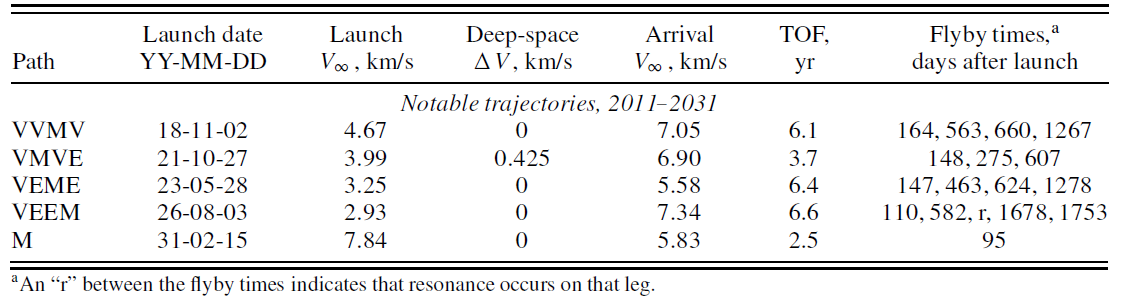
\includegraphics[width=1\textwidth]{figures/Orbiter/traj.png}
\caption{$\Delta V$ – optimized Jupiter gravity assisted trajectories from 2011 to 2031. \cite{petropoulos2000a}}\label{fig:grav_ass_traj}
\end{figure}

\noindent
Selecting a favourable flyby path is a factor of minimizing cost and at the same time maximizing payload and time of flight (TOF) time. Also, reducing arrival hyperbolic speed ($V_{\infty}$) means less excess speed for the Jupiter orbiter insertion burn to take out and so less fuel needed for the burn. As we can see from figure 3.1, an opportunity of reaching Jupiter through Venus – Earth – Mars and Earth flybys, launching in May 28, 2023 will provide the least arrival excess speed while keeping the launch $V_{\infty}$ requirement low (Launch $V_{\infty}$=3.25Km/s). The VEGA orbit was used successfully by the latest Jupiter orbiter mission, Galileo as shown in figure 3.2.

\begin{figure}[htb!]
\centering
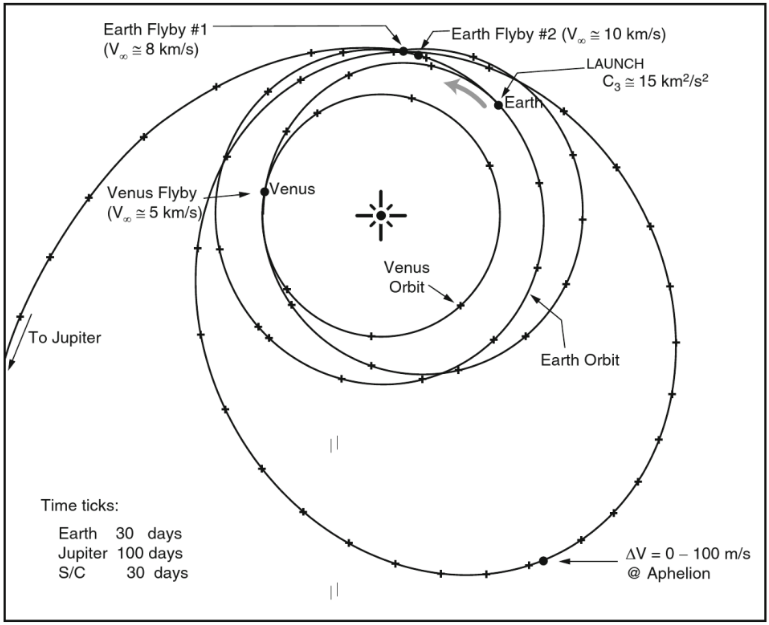
\includegraphics[width=0.8\textwidth]{figures/Orbiter/VEEGA.png}
\caption{The  VEGA orbit, used by the Galileo mission (Orbital Mechanics and Astrodynamics: Techniques and Tools for Space Missions, Gerald R. Hintz).}
\end{figure}
\section{Launch vehicle selection and evaluation}
To fulfill the mission trajectory requirement, the launch vehicle should be able to provide both the required energy and the payload capabilities of the Europa lander mission. We consided the case of two powerful launcher vehicles, the Atlas V 552 and Atlas IV Heavy by United Launch Alliance (ULA). The Atlas V family has shown solid reliability with 100 mission success since 2002 (United Launch Alliance, LLC), while providing the best match of payload mass and fairing sizes. The Atlas V 551 was used for the New Horizons mission to Pluto and Juno mission to Jupiter (one Earth flyby, TOF: 4.9 years), however the Europa lander mission will require a more massive payload to be delivered and so the Atlas V552 or even the currently more powerful rocket, the Atlas IV Heavy will be required. 

Using the required excess launch velocity of  $V_{\infty}$=3.25Km/s, we can calculate the characteristic $C_3$ energy which the rocket vehicle should provide to the payload that we want to arrive at Jupiter. This includes the full wet mass of the Europa lander mission (orbiter, lander, penetrator plus the required fuel for all phases of the mission). Using the Launch Vehicle Performance Calculator (Silverbird Astronautics \footnote{http://www.silverbirdastronautics.com/}) 
we calculate the maximum payload for an $C_3$ energy of $C_{3}=V_{\infty}^{2}=10.56 Km^2sec^{-2}$. Using the trajectory parameters from Table 3.1, the maximum payload for each rocket booster can be calculated and are shown in table \ref{tab:trajKg}.

% Table generated by Excel2LaTeX from sheet 'Sheet1'
\begin{table}[htb!]
  \centering
    \begin{tabular}{|c|r|r|r|r|r|}
    \multicolumn{6}{c}{\textbf{Maximum payload mass for the Atlas V 552 and Atlas IV Heavy boosters}} \bigstrut[b]\\
    \hline
    \textbf{Trajectory} & \multicolumn{1}{c|}{\textbf{Launch date}} & \multicolumn{1}{c|}{\textbf{TOF }} & $C_3(Km^{2}sec^{2})$ & \multicolumn{1}{c|}{\textbf{Atlas V }} & \multicolumn{1}{c|}{\textbf{Atlas IV}} \bigstrut[t]\\
    \textbf{} & \multicolumn{1}{c|}{\textbf{}} & \multicolumn{1}{c|}{\textbf{(years)}} & \multicolumn{1}{c|}{\textbf{}} & \multicolumn{1}{c|}{\textbf{552}} & \multicolumn{1}{c|}{\textbf{Heavy}} \bigstrut[b]\\
    \hline
    VMVE  & \multicolumn{1}{c|}{27-10-2021} & \multicolumn{1}{c|}{3.7} & \multicolumn{1}{c|}{15.9} & \multicolumn{1}{c|}{5181} & \multicolumn{1}{c|}{6759} \bigstrut\\
    \hline
    VEME  & \multicolumn{1}{c|}{28-05-2023} & \multicolumn{1}{c|}{6.4} & \multicolumn{1}{c|}{10.56} & \multicolumn{1}{c|}{\textbf{5648}} & \multicolumn{1}{c|}{\textbf{7389}} \bigstrut\\
    \hline
    VEEM  & \multicolumn{1}{c|}{3/8/2026} & \multicolumn{1}{c|}{6.6} & \multicolumn{1}{c|}{8.58} & \multicolumn{1}{c|}{5830} & \multicolumn{1}{c|}{7638} \bigstrut\\
    \hline
    \end{tabular}%
    \caption{Mass calculated in the 95\% confidence using Launch Vehicle Performance Calculator, Silverbird Astronautics.}
  \label{tab:trajKg}%
\end{table}%

\begin{figure}[htb!]
\centering
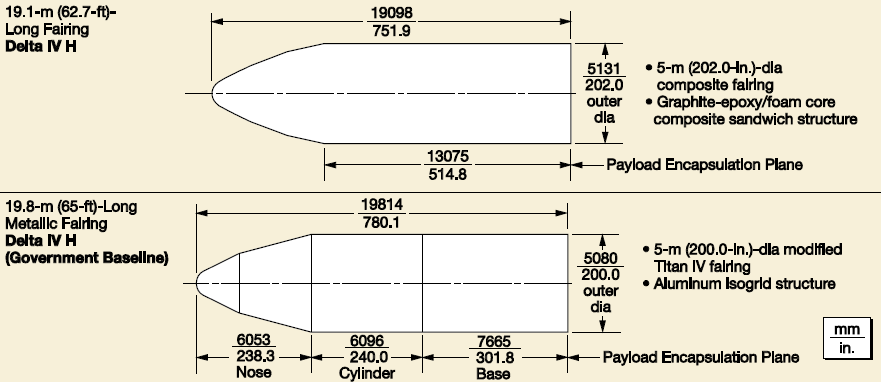
\includegraphics[width=0.8\textwidth]{figures/Orbiter/fairingsIV.png}
\caption{Atlas IV Heavy, fairing options dimentions \cite{Atlasm}.}
\end{figure}
\newpage
\subsection*{Payload dimensional considerations}
The physical dimensions of the spacecraft are limited by the launcher fairing options. The Atlas V and IV booster’s fairing options and a rocket's comparison view can be seen in figure \ref{fig:fairings}.
\begin{figure}[htb!]
    \centering
    \captionsetup[subfigure]{width=0.45\textwidth}
    \subfloat[United Launch Alliance fairing options (Delta IV Launch Services User‘s Guide, June 2013).\cite{Atlasm}]{
        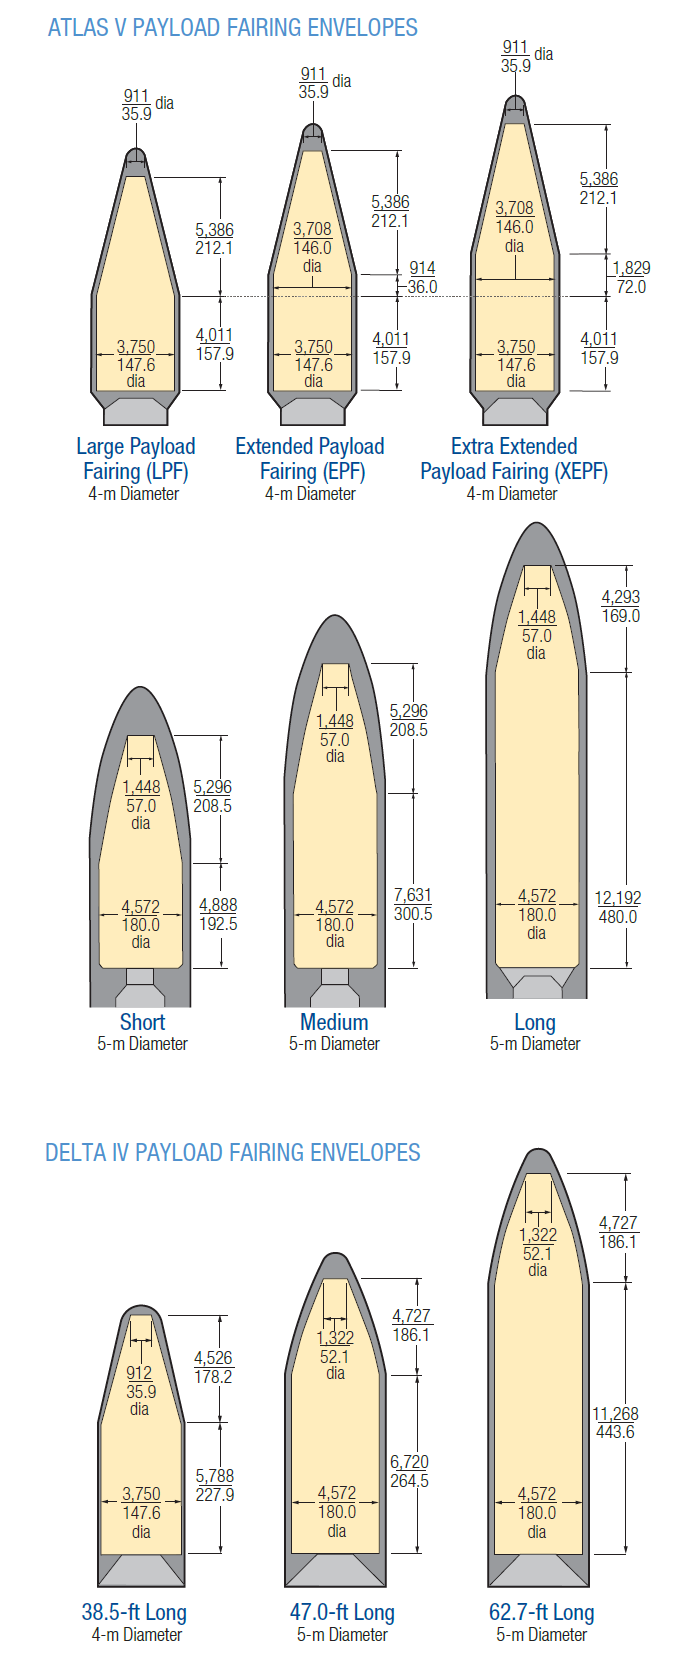
\includegraphics[width=0.48\textwidth]{figures/Orbiter/fairings.png}
        \label{fig:fairings_atlasiv}
    }
    \subfloat[Atlas V 552 and Atlas IV Heavy comparison (Delta IV Launch Services User‘s Guide, June 2013).\cite{Atlasm}]{
        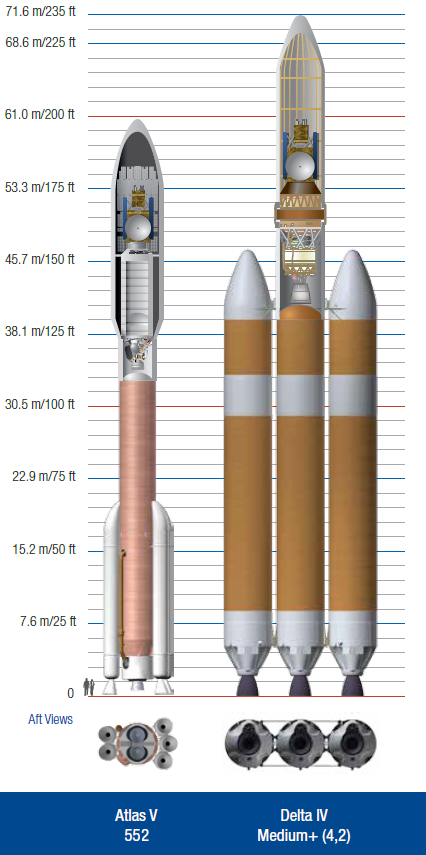
\includegraphics[width=0.48\textwidth]{figures/Orbiter/launchv.png}
        \label{fig:fairings_v_iv_compare}
    }
    \caption{Fairing Options}\label{fig:fairings}
\end{figure}
\section{Launch environment}
Launch is a mission critical event that requires significant attention for mission success. During launch, the spacecraft should survive in a fast changing and rough environment. From liftoff and until main engine cutoff (MECO), the engines produce a huge amount of mechanical vibration to the whole structure of the booster and so to the spacecraft which translates to a g-load on the delicate spacecraft components. 
Furthermore, the acoustic energy should also be considered. The acoustic environment is a function of structural design of both the fairing, fairing acoustic blankets and the spacecraft. The various components of the spacecraft should be assembled having in mind their oscillatory properties in the launch environment of the specific launcher. Another field of consideration should be the thermal properties of the ascent. As the launcher ascents the friction of the atmosphere molecules in the outer shell of the spacecraft fairing will significantly increase the fairing’s surface temperature. The acoustic blankets act also as a thermal insulator in the inner part of the fairing and so prevent the spacecraft of overheating. Further heating is avoided with fairing jettison which happens when the free stream drops below 1135 $W/m^2$\cite{Atlasm}.
Atmospheric depressurization inside the fairing is also a procedure that should be done in a controlled manner using an air duct valve. As the spacecraft may be required to wait in the launch pad in the case of an aborted liftoff, and during prelaunch activities, environmental monitoring is done using A/C and Gaseous Nitrogen($GN_2$). Temperature, relative humidity and cleanness are major concern, especially in a life seeking mission where the most demanding antibacterial protective measures are taken during the years of assembly prior to launch. Moreover, the Radioisotope Nuclear Generators (RTGs) will radiate heat continuously in the fairing enclosure and so temperature regulation is of paramount significance. Last, extra attention should be given to the outgassing properties of the fairing materials due to the intense heating that takes place during the ascent. Outgas molecules from nonmetallic materials can deposit on spacecraft materials and contaminate the sensitive life seeking instruments. 
According to ULA Atlas IV regulations, the acoustic blankets are made of Melamine foam covered with carbon-filled Kapton face sheets that eliminate outgassing and cleaned with isopropyl alcohol. The airflow during ascent should vent any outgassing molecules away from the spacecraft. However, elimination of non-metallic materials in the fairing to the lowest level is necessary. Graphical representations of the above parameters are shown in the following pages from the ULA Atlas IV user guide, version June 2013. Metallic fairing option is preferred for minimizing the outgassing factor. As it can be seen from figure \ref{fig:gloads}, the maximum load of the spacecraft will be approximately 5g at maximum dynamic pressure during first stage burn. Regarding the acoustic and shock levels, an acoustic and a vibration test is necessary to simulate and test the spacecraft rigidity prior to launch. The requirements for the acoustic test are shown in figure \ref{fig:testlevels}. The vibration test should simulate both launch vibrations and separation accelerations shown also in figure \ref{fig:testlevels} for various frequencies. Isostatic joints will be used to avoid stress forces on the spacecraft due to the temperature variations and differential thermal properties of the joint materials. 
\begin{figure}[htb!]
    \centering
    \captionsetup[subfigure]{width=0.45\textwidth}
    \subfloat[Delta IV Heavy (Metallic PLF) Absolute Pressure Envelope.\cite{Atlasm}]{
        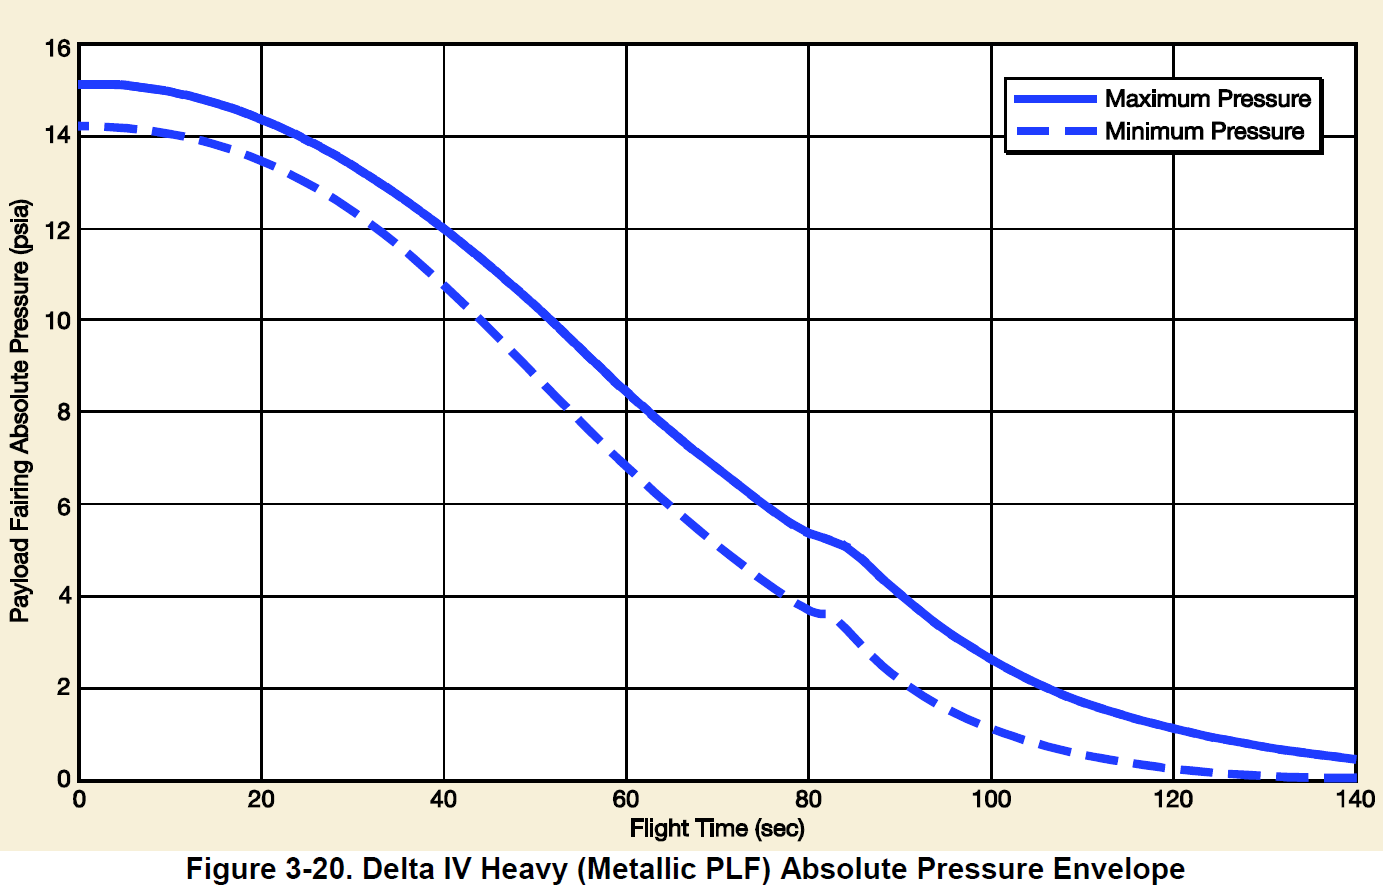
\includegraphics[width=0.48\textwidth]{figures/Orbiter/pressure.png}
        \label{fig:deltaiv_pressure_env}
    }
    \subfloat[Maximum Inner Surface Temperature - Environments to Spacecraft.\cite{Atlasm}]{
        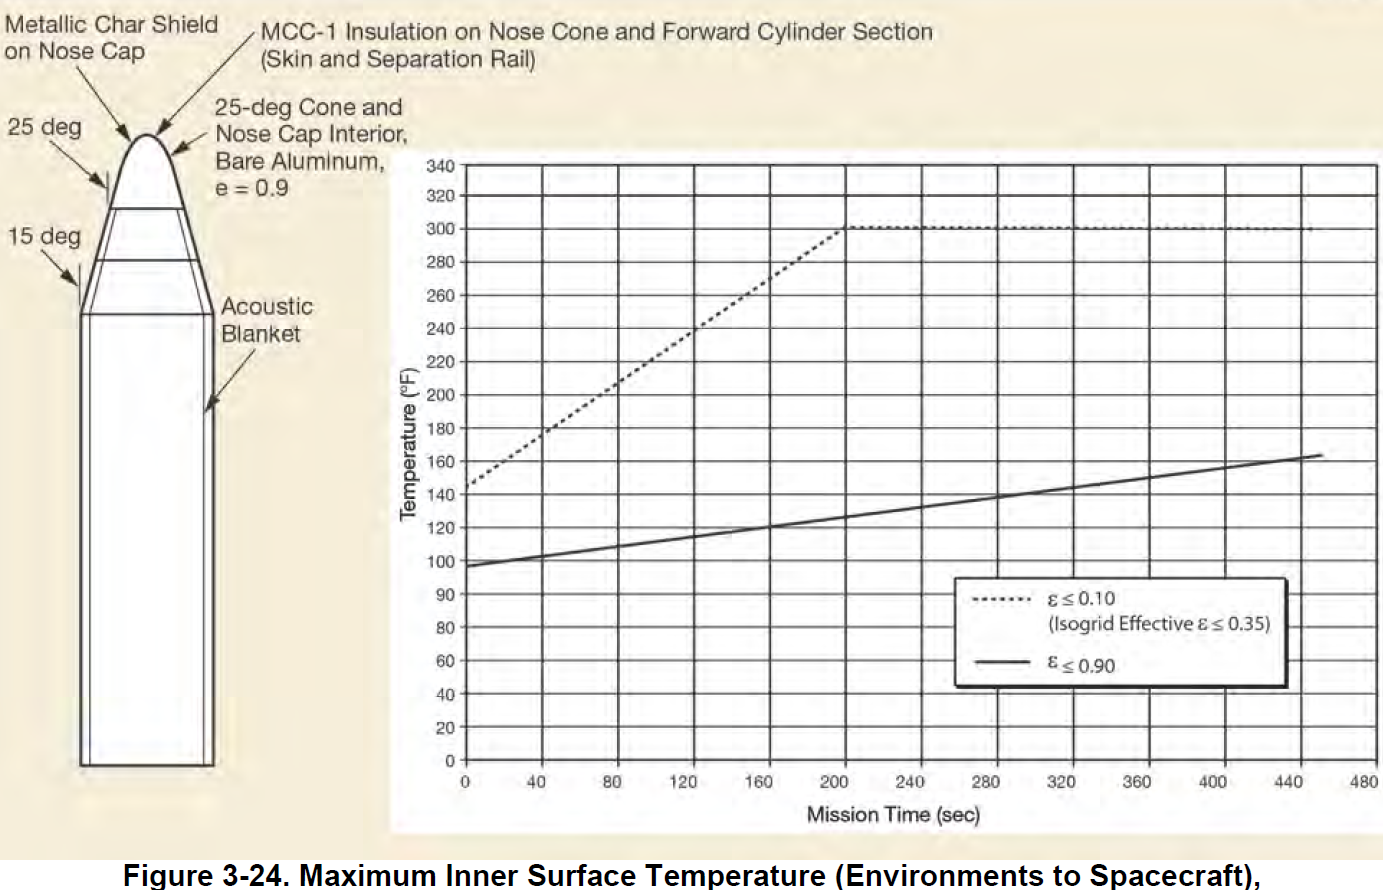
\includegraphics[width=0.48\textwidth]{figures/Orbiter/shell_temp.png}
        \label{fig:deltaiv_temp}
    }
    \caption{Pressure and temperature parameters.}\label{fig:press_temp}
\end{figure}

\begin{figure}[htb!]
    \centering
    \captionsetup[subfigure]{width=0.45\textwidth}
    \subfloat[First-Stage Burn vs. Second Stage.\cite{Atlasm}]{
        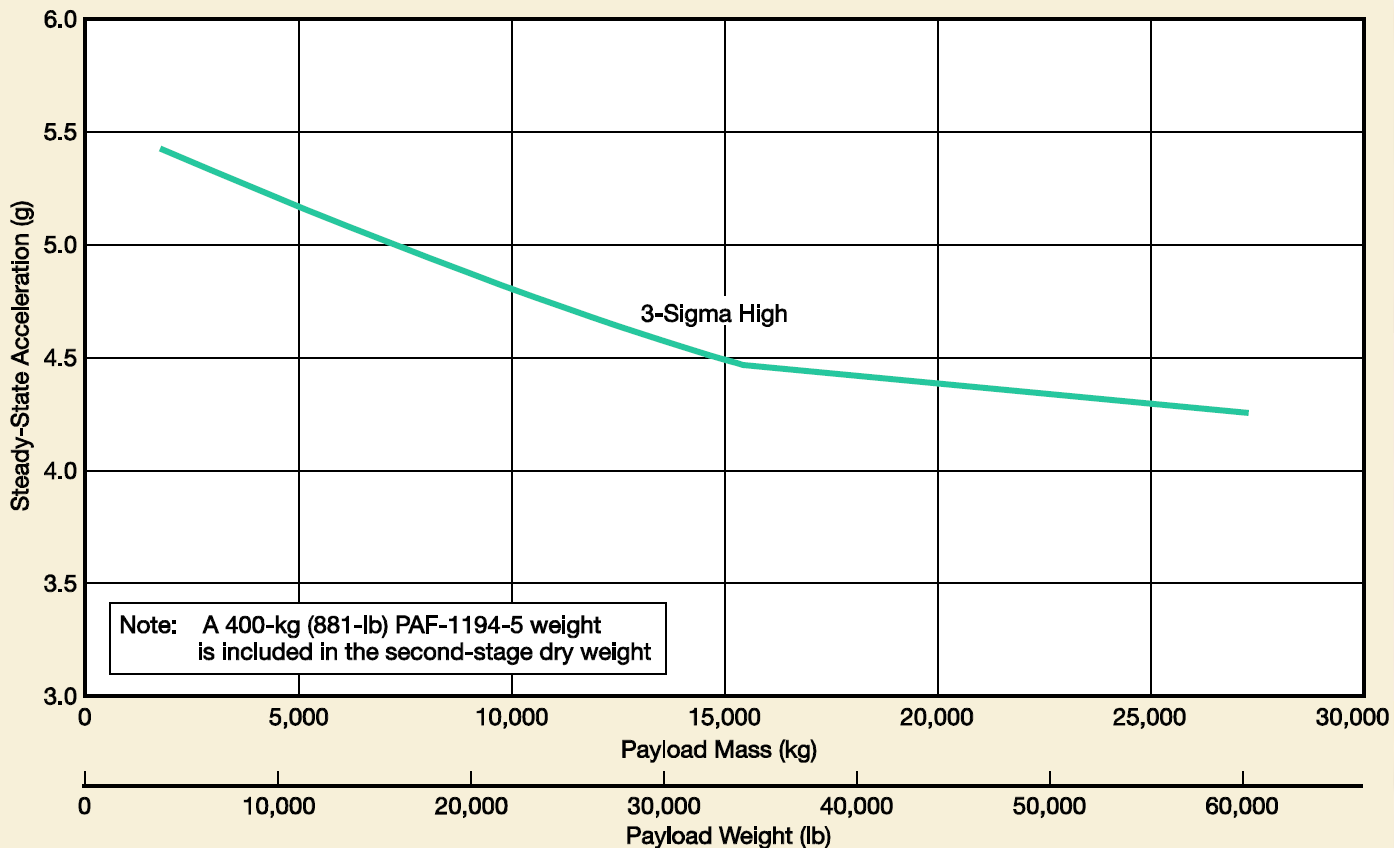
\includegraphics[width=0.48\textwidth]{figures/Orbiter/g_staging.png}
        \label{fig:gloads}
    }
    \subfloat[Second Stage Cutoff.\cite{Atlasm}]{
        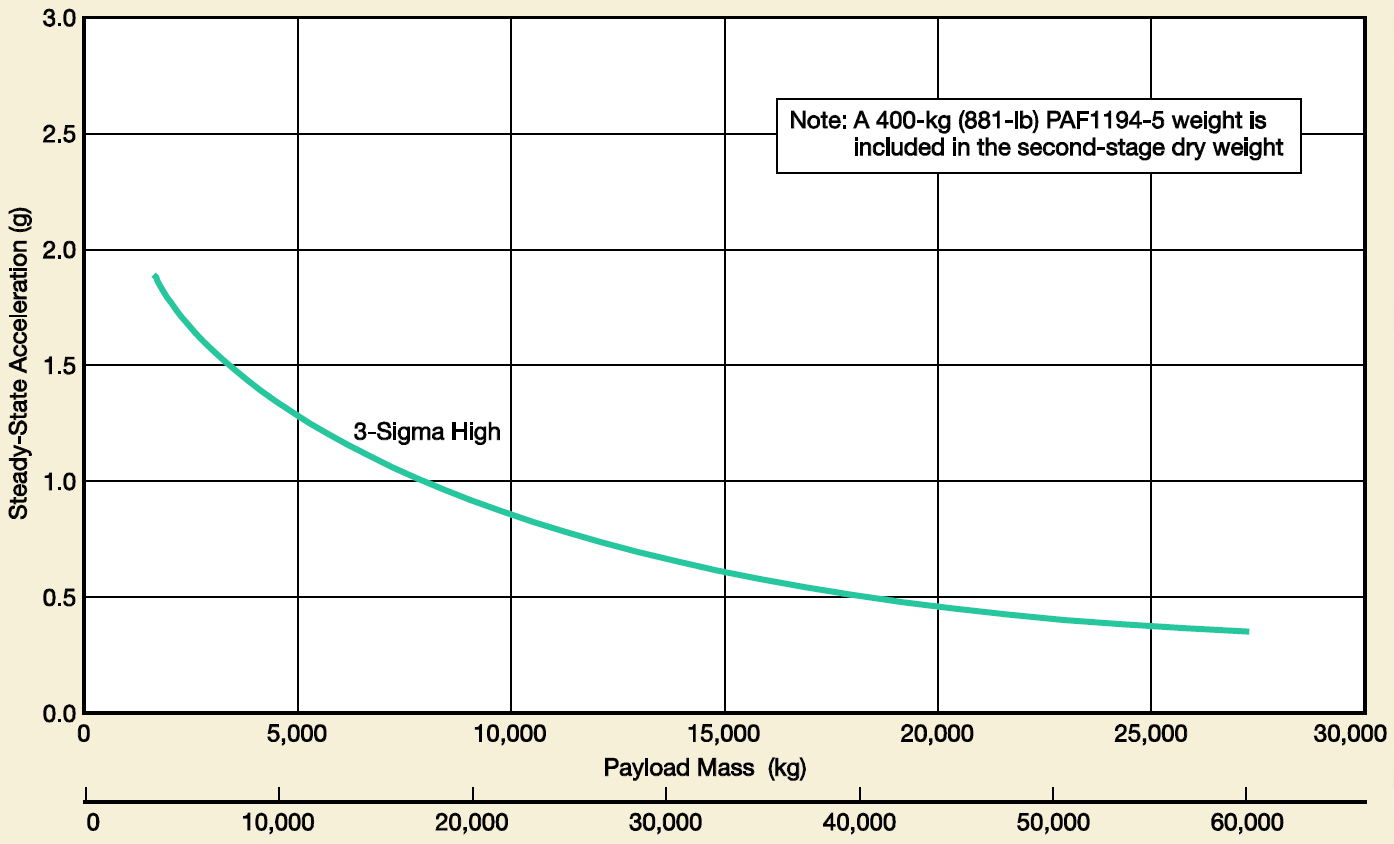
\includegraphics[width=0.48\textwidth]{figures/Orbiter/g_2ndstage.png}
        \label{fig:g_2ndstage}
    }
    \caption{Delta IV Heavy Maximum Axial Steady-State Acceleration}\label{fig:accel}
\end{figure}

\begin{figure}[htb!]
    \centering
    \captionsetup[subfigure]{width=0.45\textwidth}
    \subfloat[Maximum Spacecraft Separation Shock Level to Launch Vehicle.]{
        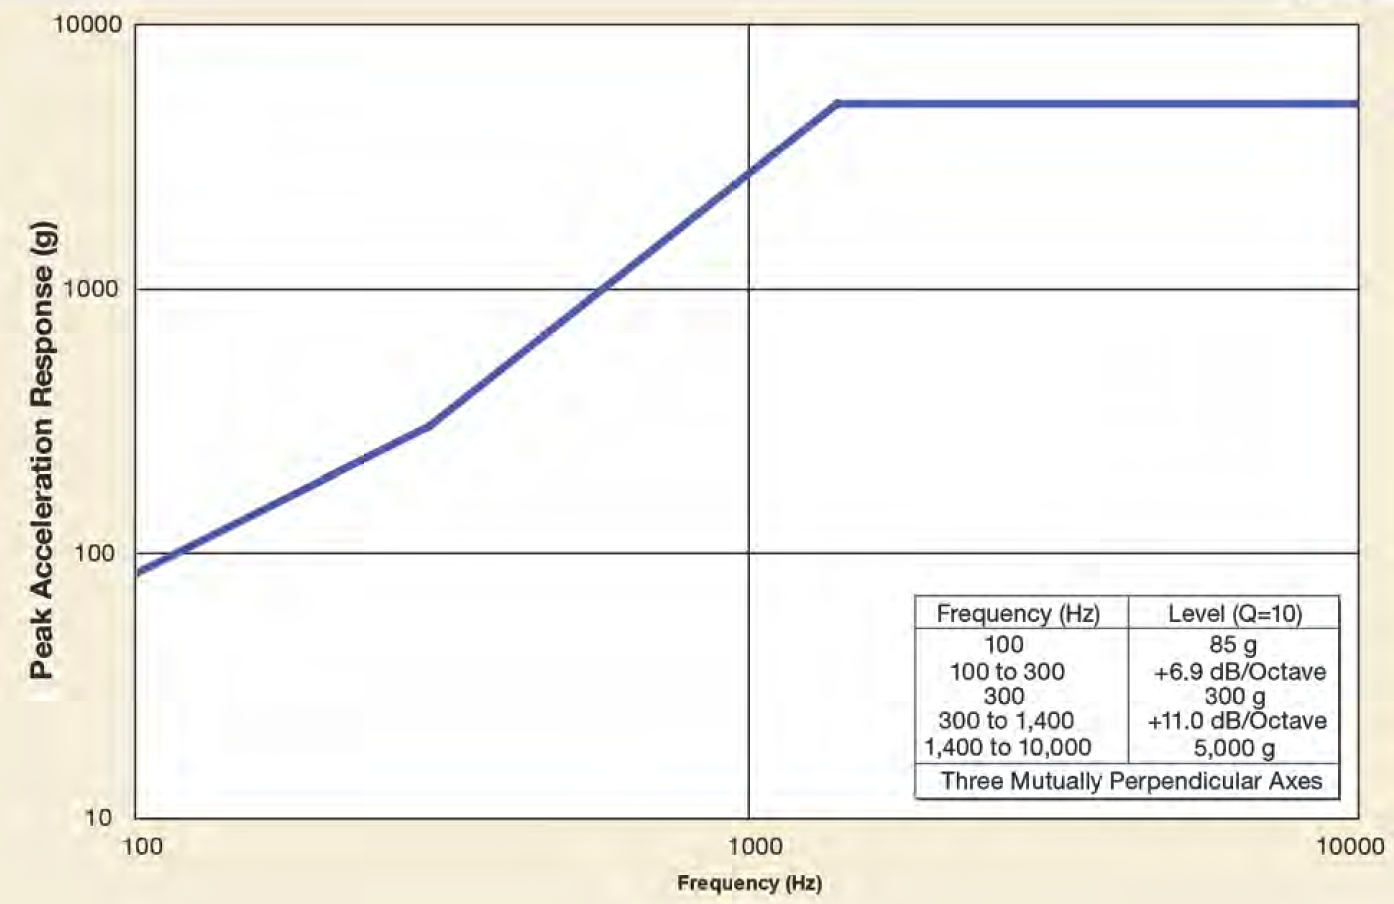
\includegraphics[width=0.48\textwidth]{figures/Orbiter/fairing_sep_resp.png}
        \label{fig:fairing_sep_resp}
    }
    \subfloat[Launch-Vehicle-Induced Payload Interface Shock Environment.]{
        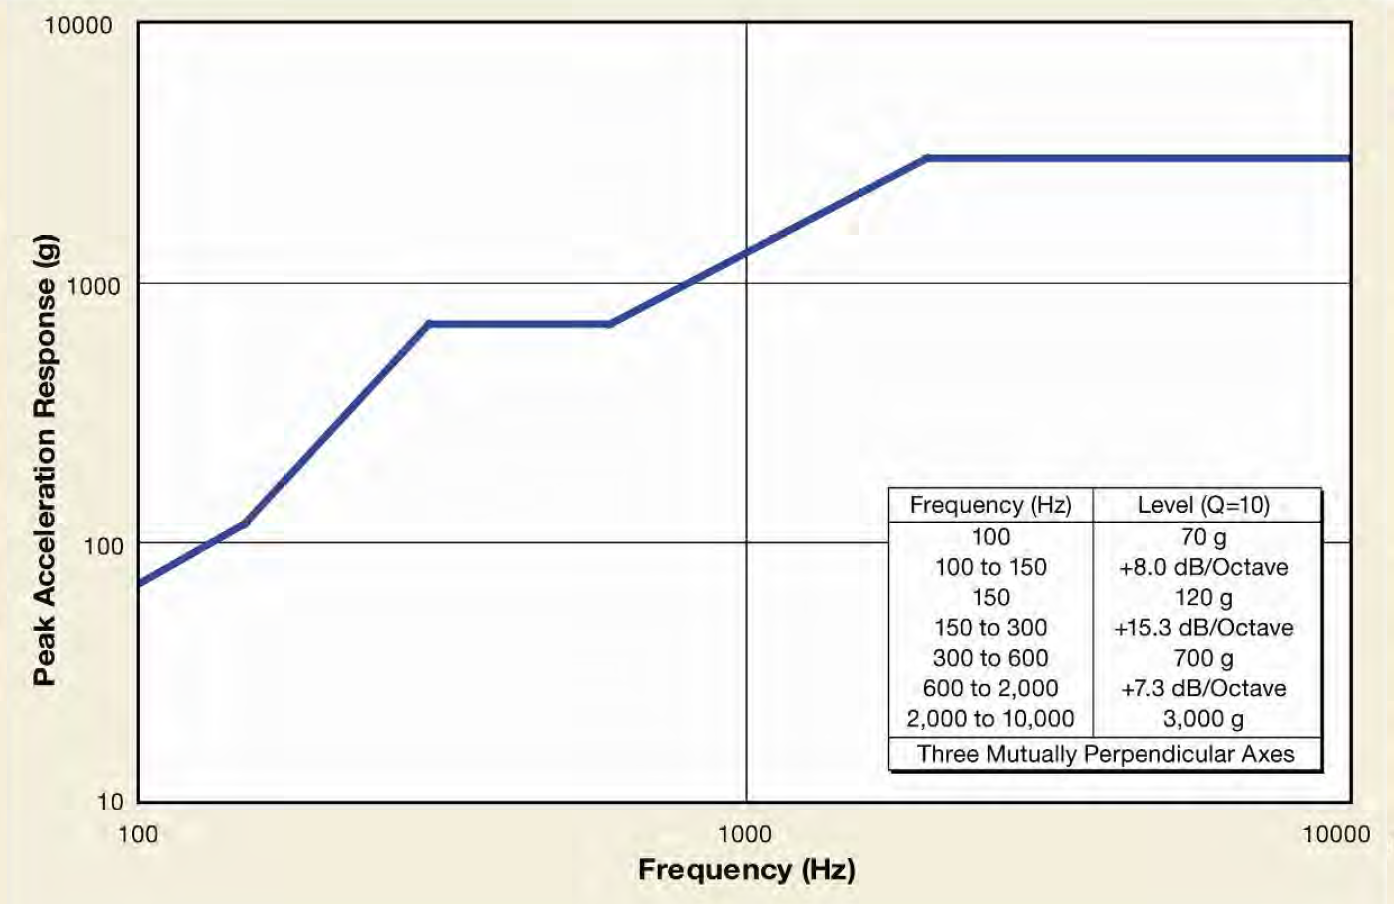
\includegraphics[width=0.48\textwidth]{figures/Orbiter/before_fair_sep.png}
        \label{fig:before_fair_sep}
    }
    \caption{Spacecraft shock environment. 1575-5 Payload Attach Fitting (95th Percentile, 50\% Confidence)\cite{Atlasm}}\label{fig:shock_env}
\end{figure}

\begin{figure}[htb!]
\centering
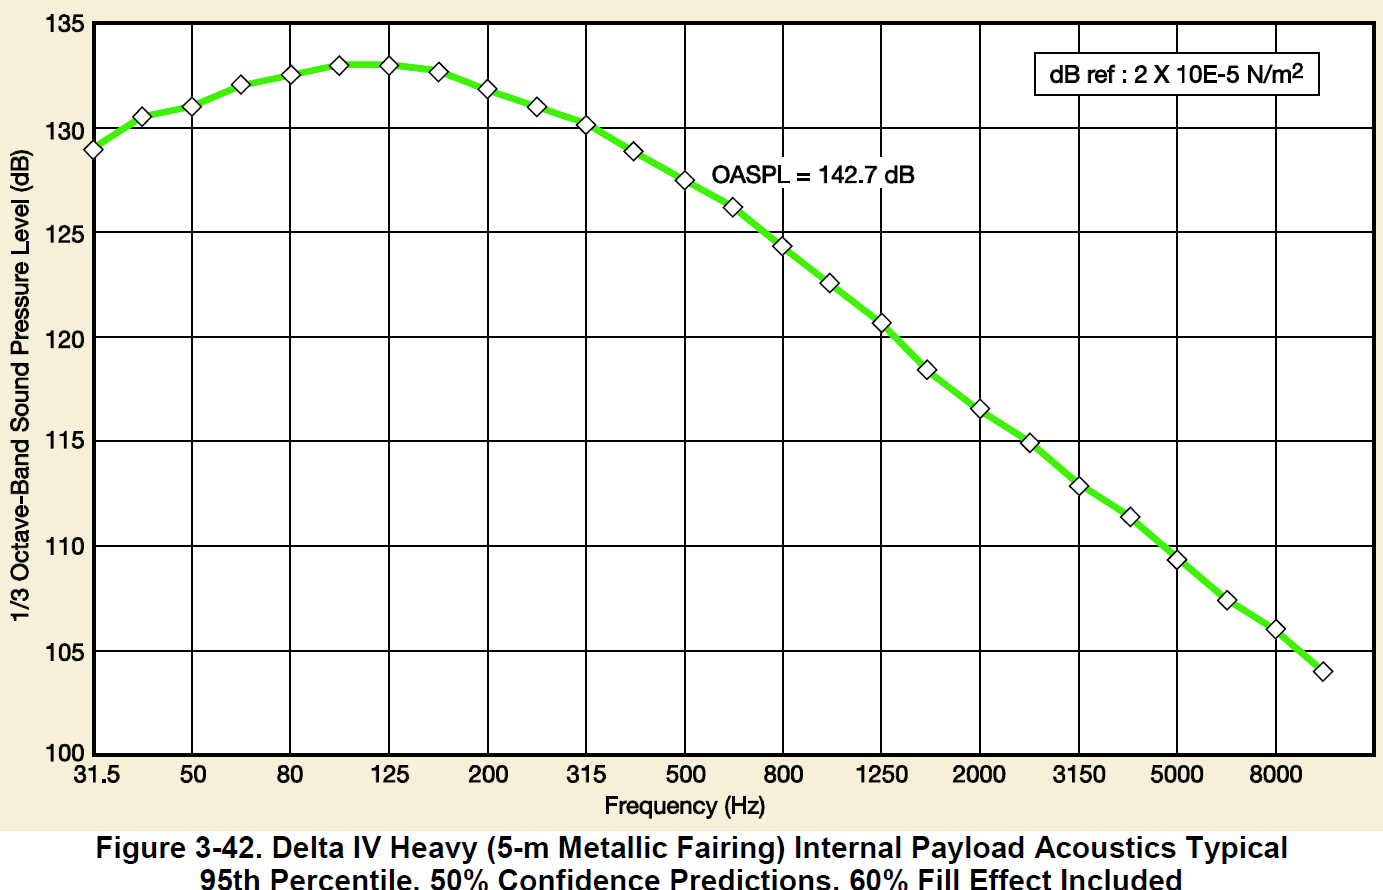
\includegraphics[scale=0.3]{figures/Orbiter/acoustics.png}
\caption{Delta IV Heavy (5-m Metallic Fairing) Internal Payl. Acoustics Typical 95th Percentile, 50\% Conf. Predictions, 60\% Fill Effect Included\cite{Atlasm}.}
\end{figure}

\begin{figure}[htb!]
\centering
\includegraphics[scale=0.3]{figures/Orbiter/acceptancelevels.png}
\caption{Acoustic and vibration test requirements\cite{Atlasm}.}
\label{fig:testlevels}
\end{figure}

\section{Cruise phase}
The cruise phase is the stage the spacecraft spends between launch and Jupiter arrival. During this 6.4 years period, the spacecraft should remain healthy and every system and science instrument should be designed to survive and be fully operational for the duration of its mission. 

During the cruise phase 4 flybys are planned, one from Venus, two from Earth and one from Mars. These flybys will provide the additional required $\Delta V$ to boost the apoapsis of the orbit to Jupiter's vicinity. The spacecraft will be equipped with a main engine and smaller Reaction Control System (RCS) thrusters. This propulsion system will be used to perform Trajectory Correction Maneuvres (TCM) to fine tune flyby trajectories. 

The flybys will also be used as a calibration test of the navigation and geolocalization system of the orbiter which will later be used to map Europa and find potential landing sites. As the mission is planning to flyby Europa multiple times when the Europa reconnaissance phase begins, the interplanetary flybys can be used as a useful analogy to simulate the flyby sequence and identify potential flaws before the actual mission begins. For example, small axis misalignment's of the telescope system with the star tracker’s axis can be spotted using star fields of both telescopic cameras and star trackers and so updating the rotational matrix parameters. This can be done by pointing to a known star fields. Precise knowledge of the spacecraft orientation is crucial for accurate pointing of the cameras while avoiding unintentional pointing of them to the Sun and at the same time keep pointing the high gain antenna to Earth.During cruise, all science instruments will be kept in hibernation mode to eliminate ageing degradation and potential software improvements found post launch will be addressed by software updates. Health checks of the systems will be performed many times during cruise. The cruise phase provides an additional benefit of using the telescope camera for Venus and Mars observations during the flybys as long as potential asteroid flybys on the way to Jupiter.

Special attention should be given to the thermal environment of the spacecraft during the flybys, due to the thermal heating of the inner planets which will be considerably more intense in the case of the Venus flyby. As the emitted energy is calculated using the black body radiation (given by Stefan-Boltzmann law)$L=4\pi R^2\sigma T^4$, where $\sigma$ is the Stefan-Boltzmann constant ($\sigma=5.670373\cdot 10^{-8}  Wm^{-2} K^{-4}$) and T the surface temperature and R the radius of the Sun. As the energy falls by the square of the distance from the source, it can be calculated that the highest solar energy the spacecraft will experience at Venus will be 1.9 times that of the Earth (or 2611 $W/m^2$ ). Given the extra heating from Venus high reflective atmosphere (albedo 0.90), \cite{venus_fact}, and the RTG constant heating, a shade solution should be implemented for the orbiter to keep the temperature to tolerable levels for both electronics and fuel tank temperatures. 

At a given time before Jupiter arrival (30-60 days), the high resolution camera will start an observational campaign of Jupiter’s satellites. The data will be used to update the orbital parameters of the moons and keep uncertainties of their speeds and positions to the lowest level for safety and fuel efficiency of the upcoming flybys and science mission trajectory. During cruise, the spacecraft will be using its high gain antenna pointing towards Earth, at the same time acting as a sun-shield. RTGs generated heat should be dissipated through radiators and carefully monitor fuel tank and temperatures distribution in the spacecraft.

\section{Jupiter orbit insertion phase}
After travelling for six and a half years in interplanetary space, the probe encounters Jupiter sphere of influence (48.2 million Km) (\ref{app:sphere_of_infl}). The Hofmann transfer orbit to Jupiter has provided enough energy so the apoapsis of the elliptical orbit will reach Jupiter at the same time that Jupiter is close enough to perform the JOI (Jupiter Orbit Insertion) burn. The telemetry commands for burn are expected to be sent to the spacecraft several days before closest approach. The inclination of the spacecraft incoming trajectory will be close to the Europa orbital plane which is $0.47^\circ$ to Jupiter’s moons plane and $1.79^\circ$ to the ecliptic (\footnote{Overview of Europa Facts". NASA}). That would be possible from the design of the flybys performed by the spacecraft. A number of small Trajectory Correction Maneuvers (TCM) are expected to be performed during the cruise phase to fine-tune the JOI timing and positioning parameters.

The JOI burn starts before closest approach to Jupiter, with the center of the burn happening exactly at the closest approach. Evenly distributing the timing of the burn is important for efficiently reducing the spacecraft’s orbital energy and being able to be capture into Jupiter's orbit. The spacecraft enters for the first time the magnetosphere of Jupiter at a distance of 45 to 100 $R_J$, which is the range of the subsolar point of Jupiter’s magnetopause (\footnote{The configuration of Jupiter's magnetosphere,Khurana, K.K.; Kivelson, M. G.; et al. (2004)}. and is affected by Solar activity. Arriving at solar maximum, the spacecraft will encounter the magnetosphere closer to Jupiter than in a low intensity solar wind period. The JOI burn will take place between the orbits of Europa and Ganymede as this configuration leaves open the possibility of using an initial Ganymede flyby to reduce the required delta-V for Jupiter orbit capture. At the same time, targeting a JOI burn close to Europa minimizes the requirements for a larger post orbit clean-up apoJove burn to bring the periJove of the orbit to Europa’s vicinity. Moreover, the periJove burn at this altitude avoids exposing the spacecraft to the high intensity Jovian radiation belts, the harshest region of them being within 300,000 Km from Jupiter\cite{jupiter_radiation_harsh}.

An analytical examination of the radiation environment is carried out in section \ref{sec:radiation_environment}, where SPENVIS models are used to predict the estimated doses from the high energy protons and electrons. Several minutes before the critical JOI burn take’s place, the spacecraft will re-orient itself for the retrograde burn and thus remain out of high-gain antenna contact with Earth during the duration of the burn (LOS). At that time, a smaller low gain antenna will be used to provide tone signals relaying vehicle status. 
\section{Jupiter Orbit Insertion delta-V calculation}
A limiting factor in the mission is the total payload that can be brought to Europa. Before that, the spacecraft should be captured in orbit around Jupiter. We investigate the amount of fuel such a maneuver will require, having in mind that the upper mass limit is defined by our launcher vehicle, which will be the Atlas IV Heavy with the maximum payload capability of 7389Kg as calculated in table \ref{tab:trajKg}.

The spacecraft arrives at Jupiter in a hyperbolic trajectory. Jupiter gravity becomes important at the sphere of influence radius of Jupiter \ref{app:sphere_of_infl}.
, which is around 48 million Km. The hyperbolic excess velocity can be expressed as the difference of the spacecraft trajectory at the apoapsis of its Hohmann transfer orbit $V_{SC,A}$ and Jupiter’s orbital speed $V_J$:
\begin{equation}
V_\infty=V_{SC,A}-V_J
\end{equation}

\begin{figure}[htb!]
\centering
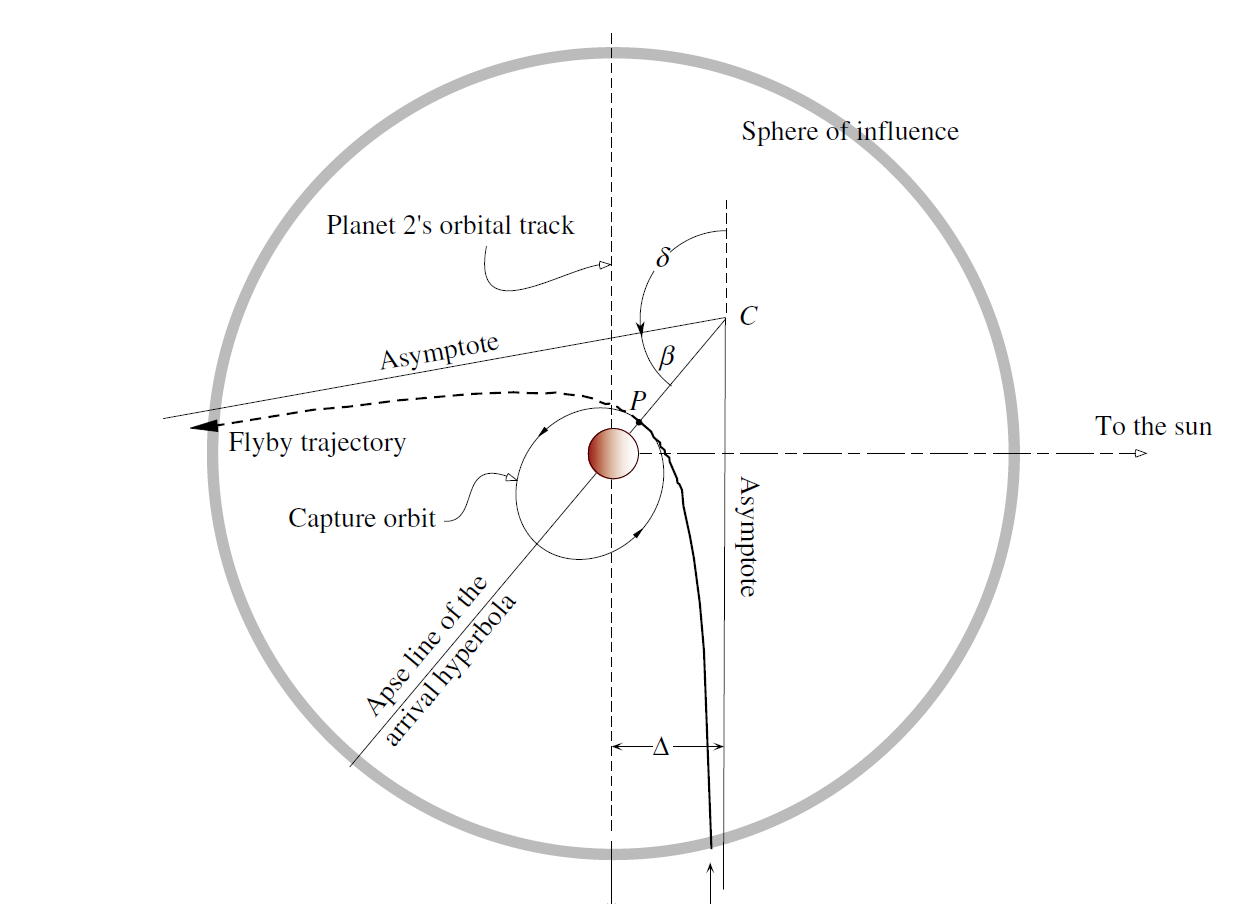
\includegraphics[scale=0.3]{figures/Orbiter/capture.png}
\caption{Incoming asymptote trajectory to Jupiter (Howard D. Curtis, Orbital Mechanics for Engineering Students).\cite{orbitals}}
\label{fig:capture}
\end{figure}

\noindent
The approach hyperbolas for a specific flyby are varying according to their aiming radius $\Delta$ as can be seen in figure \ref{fig:joihyp}. Our mission incoming asymptote will have a periapsis radius which in our case will be between the orbits of Europa and Ganymede, at a radius of $r_p=865000km$ (12$R_J$) from Jupiter. At this point, we are aiming to be captured into Jupiter orbit with the lowest amount of propellant spent. This will allow the mission to carry the maximum effective payload to Europa. 

\begin{figure}[htb!]
\centering
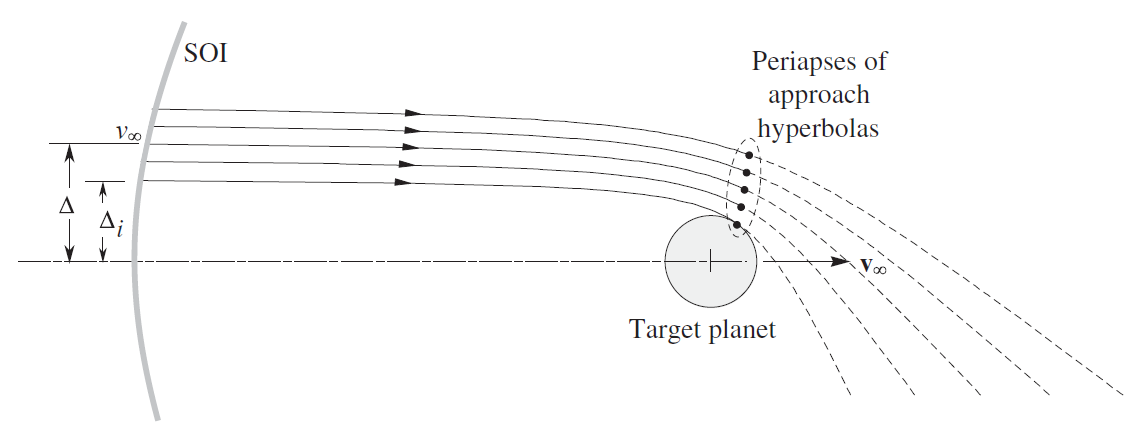
\includegraphics[scale=0.3]{figures/Orbiter/joihyp.png}
\caption{Incoming hyperbolas for varying aiming radius (Howard D. Curtis, Orbital Mechanics for Engineering Students).\cite{orbitals}}
\label{fig:joihyp}
\end{figure}

\noindent
To get into orbit, the spacecraft needs to fire its engine in the anti-velocity (retrograde) direction and remove the excess delta-V at the hyperbolic periapsis. The amount of delta-V reduction is depending on the type of capture orbit we want to achieve. In our case, the most fuel efficient option will be a highly eccentric orbit (e=0.9) around Jupiter with an orbital period of 165 days. The speed at the periapsis of hyperbolic trajectory is given by the formula:
\begin{equation}
V_{hyp,p}=\sqrt{V_{\infty}^{2}+\frac{2\mu}{r_p}}
\end{equation}
Where $\mu=GM_J$ is the gravity parameter for the Jupiter two body problem. The required speed for an elliptical Jupiter capture orbit is given by the orbital dynamics equations by the formula:
\begin{equation}
V_{capture}=\sqrt{\frac{\mu\left(1+e\right)}{r_p}}
\end{equation}
The difference of the above velocities will give us the required delta-V for Jupiter orbit capture. Note that in these calculations, the incoming asymptote of the Hohmann transfer orbit in the Jupiter reference system is parallel to Jupiter’s orbital track and so the vector subtraction of Jupiter’s orbital and spacecraft asymptotic velocities equals with the absolute values of the velocities subtraction.  Doing the delta-V calculation for the hyperbolic excess velocity given by Petropoulos et al. for the VEMEGA orbit
(\cite{petropoulos2000a}) ($V_\infty=5.58km/s$) we get:
\begin{equation}
\Delta V_{capture}=\sqrt{V_{\infty}^{2}+\frac{2\mu}{r_p}}-\sqrt{\frac{\mu\left(1+e\right)}{r_p}} = \mathbf{1.321 [km/s]}
\end{equation}
\section{Fuel mass calculation}
To calculate the fuel consumption for the required delta-V burn, we use the general rocket thrust equation:
\begin{equation}
F = \dot{m}v_e+(p_e-p_o)A_e
\end{equation}
Where the following engine parameters are required:
\begin{equation}
\begin{split}
\dot{m}&:\text{fuel mass rate}\\
v_e&:\text{equivalent velocity-exit velocity}\\
p_e&:\text{exit pressure}\\
p_o&:\text{free stream pressure}\\
A_e&:exit/nozzle \text{ area ratio}\\
\end{split}
\end{equation}

\begin{figure}[htb!]
\centering
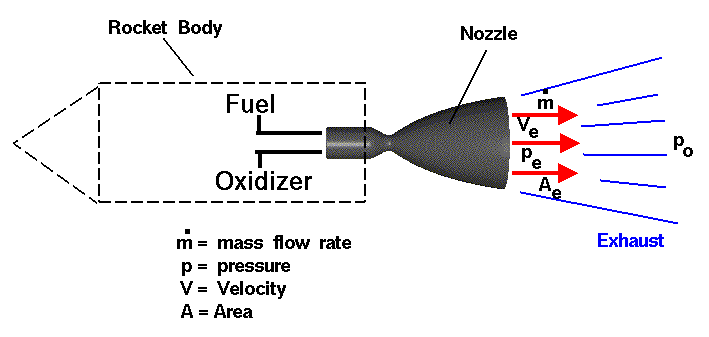
\includegraphics[scale=0.4]{figures/Orbiter/rockth.png}
\caption{Thrust equation schematic diagram (Source:NASA, GRC).\cite{rocketeq}}
\label{fig:rocketim}
\end{figure}

\noindent
Dividing the thrust equation with the mass rate, we define the equivalent velocity:
\begin{equation}
v_{eq}=\frac{F}{\dot{m}}=v_e+\frac{(p_e-p_o) A_e}{\dot{m}}
\end{equation}
Then, we define the specific impulse parameter, which describes the ratio of thrust produced to the weight of propellant, in seconds using the updated thrust equation:
\begin{equation}
I_{sp}=\frac{v_eq}{g_o} =\frac{F}{\dot{m}g_o}
\end{equation}
Thus, substituting to the thrust equation, we get the thrust written as:
\begin{equation}
F=I_{sp}\dot{m}g_o
\end{equation}
We then employ Newton’s second law of motion:
\begin{equation}
F=m\frac{du}{dt}
\end{equation}
\begin{equation}
\int_{u_o}^{u}du=-\int_{m_o}^{m}\frac{I_{sp}g_o}{m}dm
\end{equation}
So, the total velocity change can be expressed as:
\begin{equation}
\Delta v=-I_{sp}g_o ln(\frac{m}{m_o})
\end{equation}
The final mass of the spacecraft after the required delta-V change will then be:
\begin{equation}
m_{final}=m_{o}e^{-\frac{\Delta v}{v_{eq}}}
\end{equation}
\section{Spacecraft propulsion}
In order to get a realistic fuel required calculation for the JOI burn, we are using an analog of the propulsion system used in the Cassini spacecraft. The total wet mass of the Cassini-Huygens mission was 5712Kg \cite{cassini} and used two engines, one for redundancy.
Cassini's engine characteristics and the Europa Life Finder Mission are shown in the following board:

% Table generated by Excel2LaTeX from sheet 'Ark1'
\begin{table}[htb!]
  \centering
    \begin{tabular}{|c|c|c|}
    \hline
          & \textbf{Cassini} & \textbf{Europa Lander Mission} \bigstrut\\
    \hline
    Engine Thrust (N) & 440   & \textbf{500} \bigstrut\\
    \hline
    Engine Isp (s) & 308   & \textbf{300} \bigstrut\\
    \hline
    Spacecraft wet mass (Kg) & 5574  & \textbf{7300} \bigstrut\\
    \hline
    \end{tabular}%
    \caption{Cassini propulsion comparison.\cite{cassini}}
  \label{tab:propulsion}%
\end{table}%

\noindent
Using the engine thrust equations, the calculated fuel mass for the JOI burn has the requirements specified in table (\ref{tab:joi_burn_req}).

\begin{table}[htb!]
  \centering
    \begin{tabular}{|c|c|}
    \hline
    \textbf{Engine Thrust Efficiency} & 100\% \bigstrut\\
    \hline
    \textbf{DeltaV Magnitude (Km/s)} & 1321\bigstrut\\
    \hline
    \textbf{Burn duration (min)} & 262.7\bigstrut\\
    \hline
    \textbf{Fuel used (Kg)} & \textbf{2642}\bigstrut\\
    \hline
    \end{tabular}%
    \caption{JOI burn requirements}
  \label{tab:joi_burn_req}%
\end{table}%
\newpage
\section{Possibility of initial Ganymede pump-down flyby}
In order to further reduce the calculated propellant mass required for the JOI burn, there is the possibility of using an initial Ganymede flyby. A flyby at 500Km altitude from Ganymede will save about 400 Km/s of delta-V \cite{clipper} which translates to 928Kg of fuel saved for our mission. As the fuel saving is significant, the Europa Life Finder Mission will use the initial Ganymede flyby. The time coordination of the Ganymede flyby will be further redefined from the pre-arrival Jupiter moons observation campaign and the TCM burns several months before arrival to Jupiter.

\begin{table}[htb!]
  \centering
    \begin{tabular}{|c|c|c|}
    \hline
    \textbf{} & No initial Ganymede flyby & Initial Ganymede flyby \bigstrut\\
    \hline
    \textbf{Engine Thrust Efficiency} & 100\% & 100\% \bigstrut\\
    \hline
    \textbf{DeltaV Magnitude (Km/s)} & 1321  & 921 \bigstrut\\
    \hline
    \textbf{Burn duration (min)} & 262.7 & 197.6 \bigstrut\\
    \hline
    \textbf{Fuel used (Kg)} & \textbf{2642} & \textbf{1963} \bigstrut\\
    \hline
    \end{tabular}%
    \caption{JOI burn requirements with and without an initial Ganymyde pump-down flyby.}
  \label{tab:joi_burn}%
\end{table}%

\noindent
For figures (\ref{fig:joicloseup}), (\ref{fig:joifull}), the STK software was used to simulate and test our calculations for the JOI burn. Initial conditions were given: 1) the spacecraft total wet mass (7300 Kg), 2) the perijove aim radius (865000 Km), 3) burn time (262.7 min). Also the selected propulsion system was used /ref{tab:propulsion}. The The Summary report of the calculation agrees with our estimated parameters, as seen in figure (\ref{fig:stk_report1}) and (\ref{fig:stk_report2})

\begin{figure}[htb!]
\centering
\includegraphics[scale=0.25]{figures/Orbiter/JOIcloseup.png}
\caption{Simulation of the JOI burn sequence (Ifikratis Kamenidis, STK Software).}
\label{fig:joicloseup}
\end{figure}

\begin{figure}[htb!]
\centering
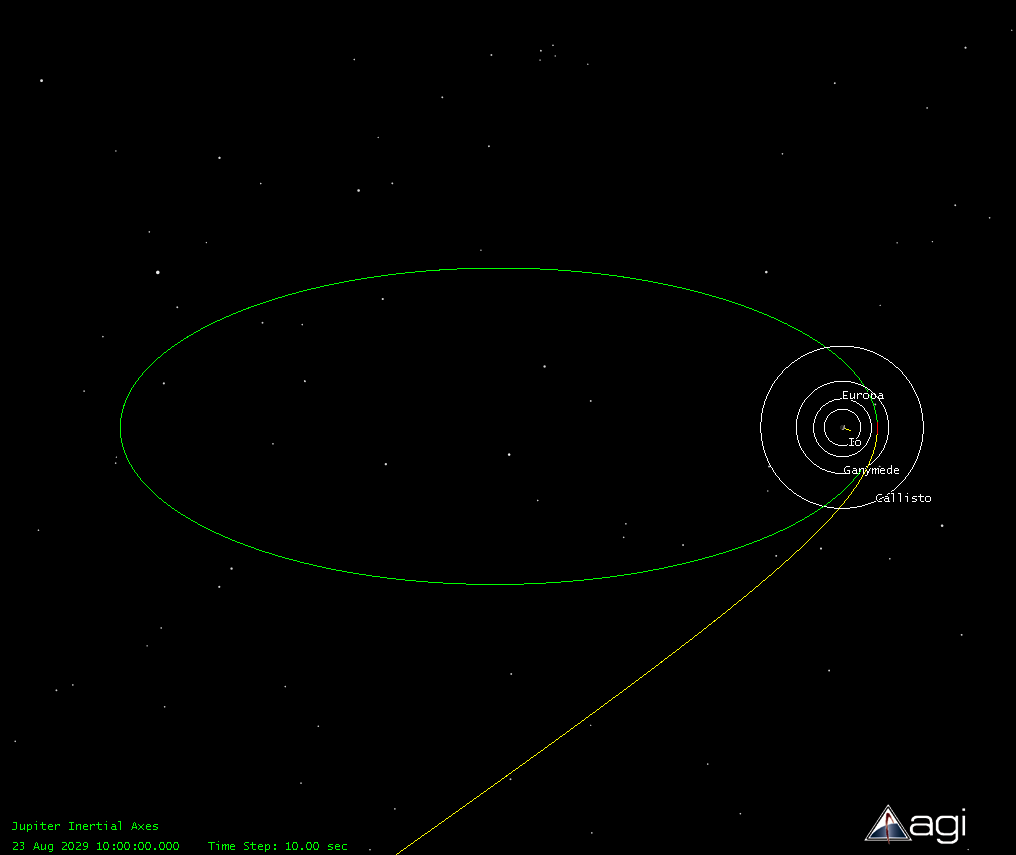
\includegraphics[scale=0.4]{figures/Orbiter/JOIfull.png}
\caption{Simulation of the JOI burn sequence and 165 days capture orbit (Ifikratis Kamenidis, STK Software).}
\label{fig:joifull}
\end{figure}

\begin{figure}[htb!]
\centering
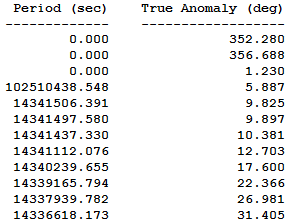
\includegraphics[scale=0.5]{figures/Orbiter/captorb.png}
\caption{STK Orbital period calculation report before and after JOI. The simulation agrees with the 165 days target initial orbit(Ifikratis Kamenidis, STK Software).}
\label{fig:stk_report1}
\end{figure}
\begin{figure}[htb!]
\centering
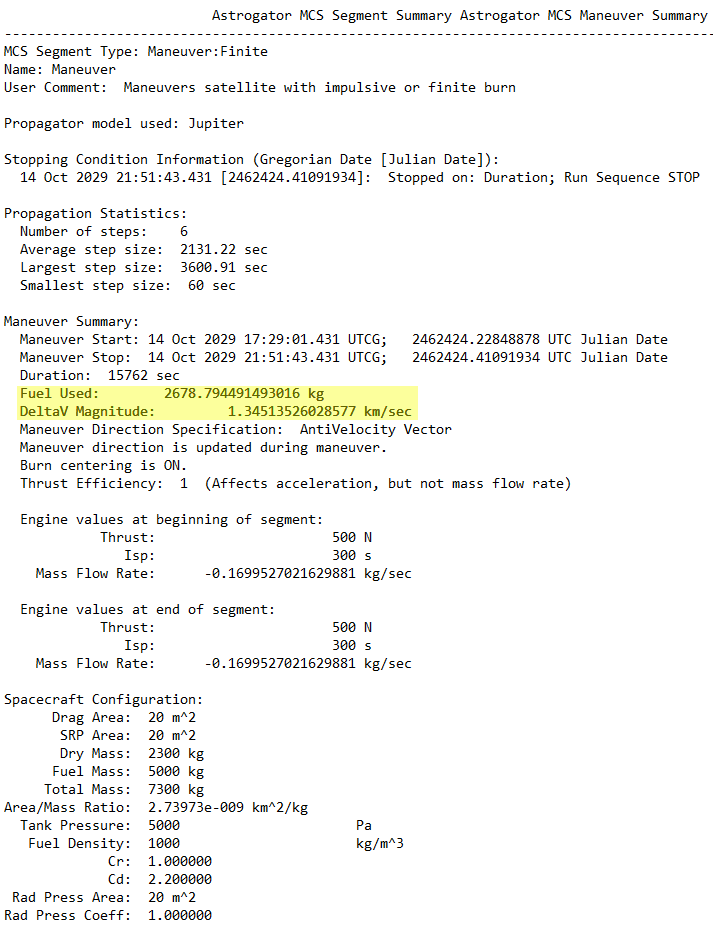
\includegraphics[scale=0.5]{figures/Orbiter/JOIres.png}
\caption{The summary report of JOI burn agrees with our predicted values.(Ifikratis Kamenidis, STK Software).}
\label{fig:stk_report2}
\end{figure}
\section{Jupiter Capture Orbit}
 The selection of the equatorial plane for the Jupiter orbit insertion was done based on the orbiter's mission goals, which is to characterise Europa’s through multiple flybys and deploy a lander into its surface. The only viable way from an orbital mechanics point of view to intercept Europa many times, achieve a good surface coverage before landing and deploy a lander using the least amount of carrying fuel is a by using a low -relative to Europa- inclination orbit around Jupiter. While a polar orbit would better avoid the high radiation lobes of the Jupiter magnetosphere, the above criteria could not be met. An orbit around Europa was ruled out based on the extremely high radiation levels. The JOI burn was designed taking into account the above orbital mission requirements while saving fuel using the opportunity of an initial Ganymede flyby. The capture orbit parameters, and especially the eccentricity of 0.6 was chosen as a realistic trade-off between orbital period and fuel required. A higher eccentricity orbit would require less fuel but would lead to a very high orbital period around Jupiter, prolonging the start of the Europa mission for more than 2 years. On the other hand a lower eccentricity orbit would spare a significant amount of fuel to lower the eccentricity.
\section{Post-Capture orbital design}
Right after the successful completion of the 197min JOI burn, the spacecraft has been captured in the initial 165 days orbit. However, the missions goal's wouldn't be achieved by staying in this long period orbit. The orbital plan is to use the more massive of the Jovian satellites, Ganymede, multiple times to slow the spacecraft down and bring it to a Europa 3:1 resonant orbit around Jupiter. For this scenario to be successful, the spacecraft should use a minimum amount of fuel to fine tune the Ganymede flybys and achieve most of the $\Delta V$ reduction from the close Ganymede encounters. 
\section{Post-Capture orbits progression analysis}
Just by letting the spacecraft orbit Jupiter in a 165 days orbit, will require significant amount of fuel to target a Ganymede flyby, as the relative positions of the spacecraft and Ganymede would be completely random. For that reason, the JOI burn and arrival time are properly targeted during cruise's TCM so that the spacecraft will pass close to Ganymede in the first inbound leg of the capture orbit just before it completes its first 165 orbit. However, the JOI burn and a potential initial Ganymede flyby create unavoidably a post-capture $\Delta V$ error. This  error would be easy to take out in the first apojove pass, targeting the first Ganymede post-orbit pump-down flyby. At this point, the amount of $\Delta V$ required to plan the Ganymede flyby is small enough (analysis follows) to easily achieve a very close Ganymede flyby and so achieve the maximum $\Delta V$ reduction. However, thinking more wisely, such a manoeuvre will not result in the maximum fuel efficiency in the long term. The resulting orbit will then need a significant amount of fuel to plan a next Ganymede (or other moon) flyby, as the orbits will again be chaotic. Spending a huge amount of fuel will unpredictably add mass to the mission while on the other hand, waiting for many orbits for a next opportunity will shift the mission lifetime and risk its successful completion, mainly because of the accumulating radiation of Jupiter's magnetosphere.

It is evident that a more ahead-planning scenario is required. We solve this problem by performing the initial Ganymede flyby in a more reasonable way. Instead of trying to achieve the maximum $\Delta V$ reduction, we plan the first Ganymede flyby in the appropriate aiming radius for a resulting Ganymede resonant orbit. By doing so, we make sure that the next orbit will not be random, but will have an orbital period which will be an integral multiple of Ganymede's orbit around Jupiter (Ganymede resonant orbit). This coherence, assures that the spacecraft can use Ganymede again for a further $\Delta V$ reduction in the next orbit with minimum fuel required. By repeating the same scheme for the 2nd Ganymede flyby, the spacecraft is again on track for a next flyby. Any excess, post flyby $\Delta V$ is managed in the apojove pass, where a small burn is performed to fine-tune the upcoming flyby. The above orbital design will allow the spacecraft to flyby Ganymede every time with the least amount of fuel. After an achieved resonance of 4:1, a flyby with Europa is within reach, and by performing small burns and a pi-transfer Ganymyed flyby, the final Europa resonance orbit will be achieved. 
\newpage
\section{Post-Capture and fuel mass calculations}
In order to test the post-capture orbits scenario viability and perform a detailed analysis of the fuel required for the correction manoeuvres, the STK software (version 10.1.3), a physics-based software geometry engine. For the orbits simulations the Astrogator (v10.0) extension was used. 

Except Jupiter, the four largest Jovian moons gravity models was used in the simulation, to accurately simulate perturbation effects in the orbits evolution. A 7th order Runge-Kutta-Fehlberg integrator with 8th order error control with 1 sec minimum stepsize was used to propagate the spacecraft's motion in Jupiter's gravity field as well as when inside the Sphere of Influence of Ganymede and Europa, when their specific gravity fields were used (\ref{app:sphere_of_infl}). The gravity fields used can be seen in table (\ref{tab:gravf}). Furthermore, a spherical solar radiation pressure (SRP) is used with a dual-cone shadow model.

% Table generated by Excel2LaTeX from sheet 'Sheet1'
\begin{table}[htb!]
  \centering
    \begin{tabular}{|c|c|c|c|}
    \hline
    \multicolumn{4}{|c|}{\textbf{Gravity models}} \bigstrut\\
    \hline
    \textbf{Object} & \textbf{Gravity Model} & \textbf{Degree} & \textbf{Order} \bigstrut\\
    \hline
    \textbf{Jupiter} & JUP230.grv & 6     &  \bigstrut\\
    \hline
    \textbf{Io} & JUP230.grv & 6     &  \bigstrut\\
    \hline
    \textbf{Europa} & Science1998.grv & 4     & 2 \bigstrut\\
    \hline
    \textbf{Ganymede} & Nature1996.grv & 4     & 2 \bigstrut\\
    \hline
    \textbf{Callisto} & JUP230.grv & 6     &  \bigstrut\\
    \hline
    \end{tabular}%
    \caption{Gravity models used in simulation(source: NASA, Horizons, NAIF).\cite{Gravm}}\label{tab:gravf}
\end{table}%

\noindent
In order to perform the required orbits and manoeuvres calculations by the simulation engine, a series of commands are written in a logical sequence. The software uses a differential corrector to solve a problem of initial conditions, given a set of orbital goals. 
The core of the commands can be synopsised in the following sequence:

\begin{itemize}
  \item Propagate at orbit apojove
  \item Initiate burn - 3 degrees of freedom
  \item Propagate at Ganymede Sphere of Influence radius
  \item Target flyby B-plane - specific BdotR, BdotT goals are set
  \item Propagate at apoJove
\end{itemize}

\noindent
At the end of each iteration, the resulting orbital period is checked. $B\cdot R$ and $B\cdot T$ targets are altered until the desired orbital period is achieved. Then, the same iteration sequence is run for calculating the upcoming Ganymede flyby. The achieved resonances of orbit two, three and four (orbit one equals to capture orbit) are 9:1, 6:1 and 3:1 respectively. 
Table (\ref{tab:boardm}) shows an overview of the apoJove burns and flyby $\Delta V$ parameters. Assumed 5426Kg wet mass after JOI burn in the Ganymede initial pump-down scenario. The new wet mass after a burn is always taken into account in the calculations. Engine ISP=300s and Engine thrust=500N. OX-BX indicate the apoJove burns, while with GX and EX are noted the in sequence Ganymede and Europa flybys.

% Here, I want the table to appear after the text above, but its not
%one second
% Table generated by Excel2LaTeX from sheet 'Sheet1'
\begin{table}[htb!]
  \centering
    \begin{tabular}{|r|r|r|r|r|}
    \hline
          & \boldmath{}\textbf{$\Delta V (m/s)$}\unboldmath{} & \textbf{Burn time(s)} & \textbf{Fuel used (Kg)} & \textbf{Range (Km)} \bigstrut\\
    \hline
    \multicolumn{1}{|c|}{\textbf{O1-B1}} & \multicolumn{1}{c|}{4.409015} & \multicolumn{1}{c|}{29.926} & \multicolumn{1}{c|}{8.114} & \multicolumn{1}{c|}{} \bigstrut\\
    \hline
    \multicolumn{1}{|c|}{\textbf{G1}} & \multicolumn{1}{c|}{794.84} & \multicolumn{1}{c|}{} & \multicolumn{1}{c|}{} & \multicolumn{1}{c|}{2268} \bigstrut\\
    \hline
    \multicolumn{1}{|c|}{\textbf{O2-B2}} & \multicolumn{1}{c|}{0.724688} & \multicolumn{1}{c|}{4.919} & \multicolumn{1}{c|}{1.334} & \multicolumn{1}{c|}{} \bigstrut\\
    \hline
    \multicolumn{1}{|c|}{\textbf{G2}} & \multicolumn{1}{c|}{494.89} & \multicolumn{1}{c|}{} & \multicolumn{1}{c|}{} & \multicolumn{1}{c|}{3189} \bigstrut\\
    \hline
    \multicolumn{1}{|c|}{\textbf{O3-B3}} & \multicolumn{1}{c|}{4.197475} & \multicolumn{1}{c|}{28.49} & \multicolumn{1}{c|}{7.725} & \multicolumn{1}{c|}{} \bigstrut\\
    \hline
    \multicolumn{1}{|c|}{\textbf{G3}} & \multicolumn{1}{c|}{1223.24} & \multicolumn{1}{c|}{} & \multicolumn{1}{c|}{} & \multicolumn{1}{c|}{489} \bigstrut\\
    \hline
    \multicolumn{1}{|c|}{\textbf{O4-B4}} & \multicolumn{1}{c|}{1.180696} & \multicolumn{1}{c|}{8.014} & \multicolumn{1}{c|}{2.17} & \multicolumn{1}{c|}{} \bigstrut\\
    \hline
    \multicolumn{1}{|c|}{\textbf{G4}} & \multicolumn{1}{c|}{1080.2} & \multicolumn{1}{c|}{} & \multicolumn{1}{c|}{} & \multicolumn{1}{c|}{497} \bigstrut\\
    \hline
    \multicolumn{1}{|c|}{\textbf{O5-B5}} & \multicolumn{1}{c|}{103.7305} & \multicolumn{1}{c|}{1146} & \multicolumn{1}{c|}{187.376} & \multicolumn{1}{c|}{} \bigstrut\\
    \hline
    \multicolumn{1}{|c|}{\textbf{E1}} & \multicolumn{1}{c|}{804.61} & \multicolumn{1}{c|}{} & \multicolumn{1}{c|}{} & \multicolumn{1}{c|}{627} \bigstrut\\
    \hline
    \multicolumn{1}{|c|}{\textbf{O6-B6}} & \multicolumn{1}{c|}{149.8431} & \multicolumn{1}{c|}{1644} & \multicolumn{1}{c|}{256.233} & \multicolumn{1}{c|}{} \bigstrut\\
    \hline
    \multicolumn{1}{|c|}{\textbf{E2}} & \multicolumn{1}{c|}{45.98} &       & \multicolumn{1}{c|}{} & \multicolumn{1}{c|}{3771} \bigstrut\\
    \hline
    \multicolumn{1}{|c|}{\textbf{Total }} & \multicolumn{1}{c|}{4707.8} &       & \multicolumn{1}{c|}{462.952} & \multicolumn{1}{c|}{} \bigstrut\\
    \hline
    \end{tabular}%
    \caption{Resulting burn parameters for post-Jupiter capture orbits progression.}
  \label{tab:boardm}%
\end{table}%

\begin{figure}[htb!]
\centering
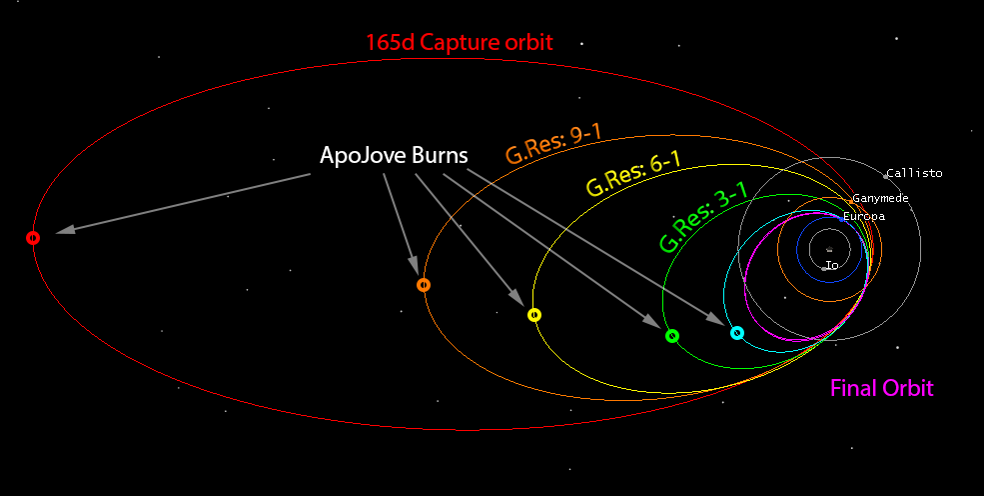
\includegraphics[width=\textwidth]{figures/Orbiter/orbits.png}
\caption{Orbits evolution from JOI to Europa target 3:1 resonance orbit. (Ifikratis Kamenidis, STK Software).}\label{fig:orbits_resonance}
\end{figure}
\begin{description}[align=left]
\item [Post-capture orbital design]\hfill \\
An animation of the post-capture orbital design can be seen at:

\url{https://www.youtube.com/watch?v=sUmYL08Vr14}
\item [Ganymede Flyby]\hfill \\
Also, an animation of a 500Km Ganymede flyby can be seen at:

\url{https://www.youtube.com/watch?v=64JcLukSnnY}.
\end{description}
\section{Arriving at target orbit}
After the completion of the third Ganymede flyby, the forth Ganymede flyby is performed with a dual purpose. First to further reduce the apojove distance of the orbit and at the same time place the spacecraft in an orbit to intercept Europa for the first time. Meanwhile, every Ganymede flyby is lowering the perijove of the orbit, while the last Ganymede flyby brings the perijove at approximately 9.3 $R_J$ in Europa's vicinity. The first Europa flyby itself is designed to provide the necessary $\Delta V$ reduction to place the spacecraft in the target 3:1 resonant Europa orbit. For every spacecraft orbit around Jupiter, Europa make exactly three orbits. This synchronisation is key in achieving a continuous flybys in order to provide the orbiter the ability to do pre-landing reconnaissance and find the best landing site location for the lander module. After landing, the same orbit will be used to provide the communication link between the penetrator -lander and the Earth. The orbital parameters of the target orbit can be seen in table (\ref{tab:eurorb}).

% Table generated by Excel2LaTeX from sheet 'Sheet1'
\begin{table}[htb!]
  \centering
    \begin{tabular}{|c|c|}
    \hline
    Semi-major axis (Km) & \textbf{1,392,748} \bigstrut\\
    \hline
    PeriJove (Km) & \textbf{662,300} \bigstrut\\
    \hline
    ApoJove (Km) & \textbf{2,525,000} \bigstrut\\
    \hline
    Eccentricity & \textbf{0.5244} \bigstrut\\
    \hline
    Inclination ($^\circ)$ & \textbf{3.816} \bigstrut\\
    \hline
    Period (days) & \textbf{10.6} \bigstrut\\
    \hline
    TID under 2cm of Al (krad/month) & \textbf{5.2} \bigstrut\\
    \hline
    Europa flyby relative $\Delta V$(Km/s) & \textbf{3.3} \bigstrut\\
    \hline
    \end{tabular}%
    \caption{Europa 3:1 resonant orbit parameters.}
  \label{tab:eurorb}%
\end{table}%
\begin{figure}[htb!]
\centering
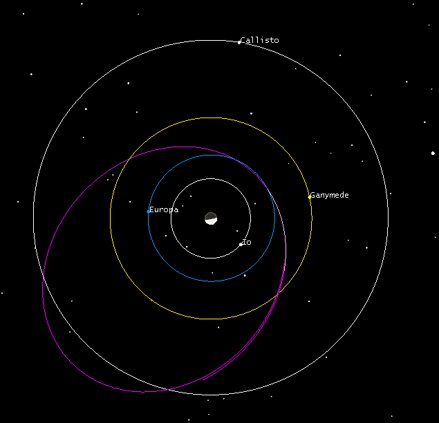
\includegraphics[scale=1]{figures/Orbiter/europares.png}
\caption{Europa 3:1 resonant orbit (Ifikratis Kamenidis, STK Software).}
\end{figure}
\section{Perturbations and orbit sustainability}
Europa's mass is significant enough to alter the spacecraft's trajectory every time it flies by the moon. The gravity assist was useful for the initial pump-down and orbital decay of the capture orbit as explained in the previous chapter. However, in the case of the target orbit, unavoidably a $\Delta V$ change will occur after every flyby. As a result, the apojove radius will now change, hence the orbital period and the 3:1 resonance synchronization. An apojove burn will be necessary in every orbit to keep the spacecraft in the resonant trajectory. In that case the amount of fuel required will be very large. Moreover, besides sustaining the orbit the goal of the orbiter's flyby is to map the surface prior to landing, and so a method of placing the groundtrack of a hyperbolic orbit over desired latitudes and longitudes has been developed by NASA \cite{cotseq}. 

The flyby sequence called "Crank-over-the-top Sequence" (COT) and was used bt the Cassini mission for the Titan flybys. The technique is implemented by cranking the inclination of the orbit starting from a n equatorial point and arriving at a maximum inclination ($i_{max}$). The incoming and outcoming v-infinity velocities have the same pump angle (\ref{fig:pump_a}).
and the total $\Delta V$ is perpendicular to the moon velocity (\ref{fig:cotgeo}). 
%\todo[inline]{graphs 5.19 & 5.20 do not appear here}

\begin{figure}[htb!]
    \centering
    \captionsetup[subfigure]{width=0.45\textwidth}
    \subfloat[Pump angle \cite{cotseq}.]{
        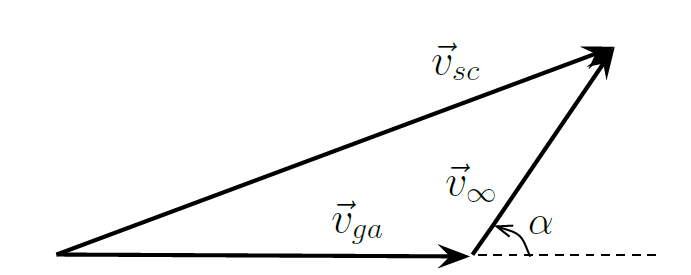
\includegraphics[width=.48\textwidth]{figures/Orbiter/pumpa.png}
        \label{fig:pump_a}
    }
    \subfloat[COT sequence flyby geometry \cite{cotseq}.]{
        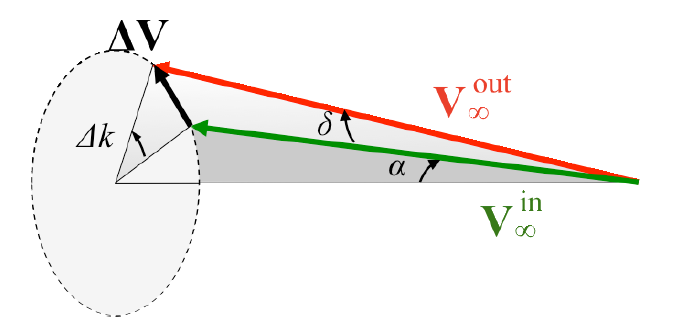
\includegraphics[width=.48\textwidth]{figures/Orbiter/flbeom.png}
        \label{fig:cotgeo}
    }
    \caption{Flyby geometry}
\end{figure}

\noindent
The COT sequence will begin will outbound flybys and cover the anti-jovian facing hemisphere of Europa which is tidally locked. The groundtracks as calculated by Brent Buffigton et al. \cite{cotseq} can be seen at figure \ref{fig:ground_tr} for a 3:1 resonant Europa COT sequence.

\begin{figure}[htb!]
\centering
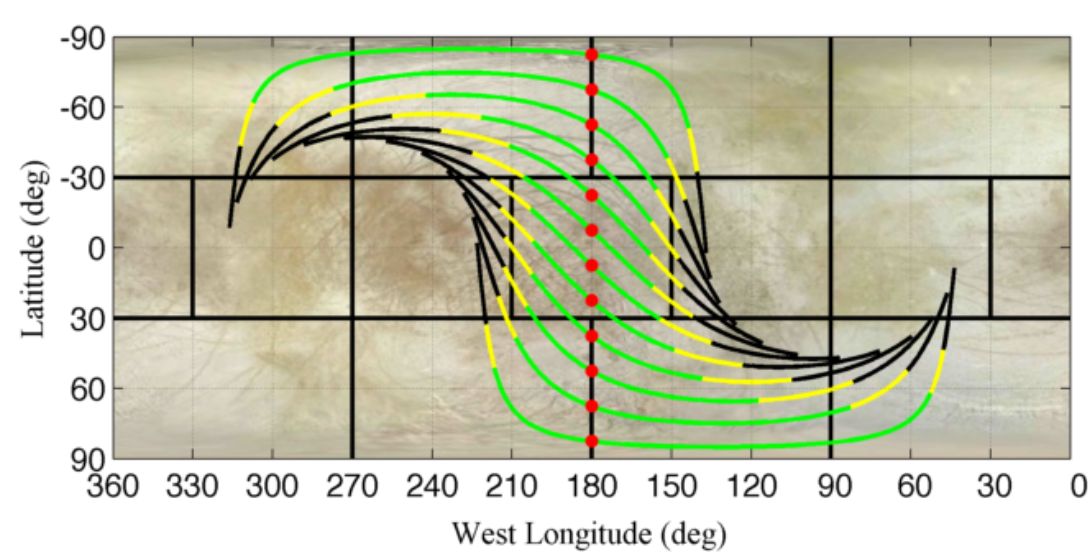
\includegraphics[scale=0.3]{figures/Orbiter/groundtr.png}
\caption{Grountracks of a COT sequence in a 3:1 resonant Europa jovian orbit \cite{cotseq}.}
\label{fig:ground_tr}
\end{figure}

\noindent
Furthermore, illumination of the moon is a crucial part of the reconnaissance as long as the landing phase. As Europa rotates around Jupiter the antijovian hemisphere will experience a 3.5 days day-night period. As shown before, the resonant orbit's perijove is also the flyby point. That means that changing the orbit's argument of periapsis ($\omega$) the line of nodes can be rotated. While at the same time keeping the resonance of the orbit, the orbiter can experience different illumination conditions on the antijovian Europa hemisphere. This shift can be achieved by using the COT sequence by cranking up the inclination and pumping down the orbit period in order to use a Europa to Ganymede pi-transfer \cite{cotseq}. As the lander requirements is find a landing spot in the antijovian hemisphere, the lighting conditions change will not require an 180 degree shift for a full moon coverage. Instead a total of 90 degree of Europa illumination rotation would be sufficient.  
\section{Flyby geometrical configuration}
As the orbiter flybys Europa, the physical orientation of the spacecraft should be maintained in order to fulfil mission goals. This is especially important in the pre-landing phase of the mission, when the ERIS (Europa Reconnaissance Imaging System) will be used to cover the surface and find candidate landing sites. 

Depending on the flyby coverate goal, a flyby can either target the leading edge hemisphere of Europa or the trailing edge. Both configurations are designed to map the antijovian facing hemisphere of Europa, as this is where a landing site is more favorable (less radiation and bigger communication windows). The leading edge hemisphere also shows a lower radiation as the fast rotation of Jupiter and so its magnetic field will hit mainly the trailing hemisphere on the 3.5 days orbit around Jupiter. Figures \ref{flyby1} and \ref{flyby2} show the two different flyby geometries. In the first case (\ref{flyby1}) the orbiter will have more time to image Europa on the outbound leg of the flyby (red) while in the second case (\ref{flyby2}) the orbiter will have more time to image Europa in the inbound leg of the flyby. Thus, the selection should be made according to flyby reconnaissance targets but also depending on the illumination of the moon the specific flyby time. Terminator areas are preferred for showing texture and shadows in interesting areas.
%\todo[inline]{pictures 5.22 and 5.23 do not appear here}
\begin{figure}[htb!]
\centering
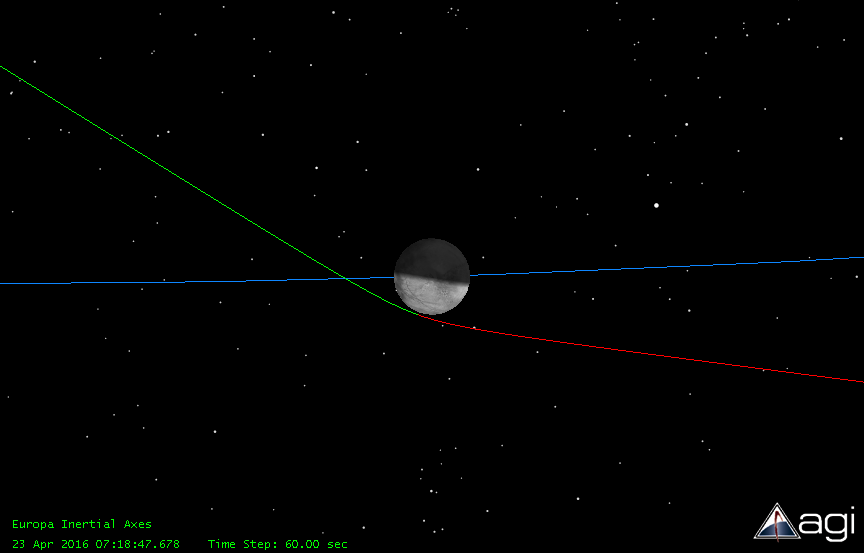
\includegraphics[width=0.9\textwidth]{figures/Orbiter/flyby1.png}
\caption{Flyby geometry targeting the leading edge antijovian hemisphere (Ifikratis Kamenidis, STK software).}
\label{flyby1}
\end{figure}

\begin{figure}[htb!]
\centering
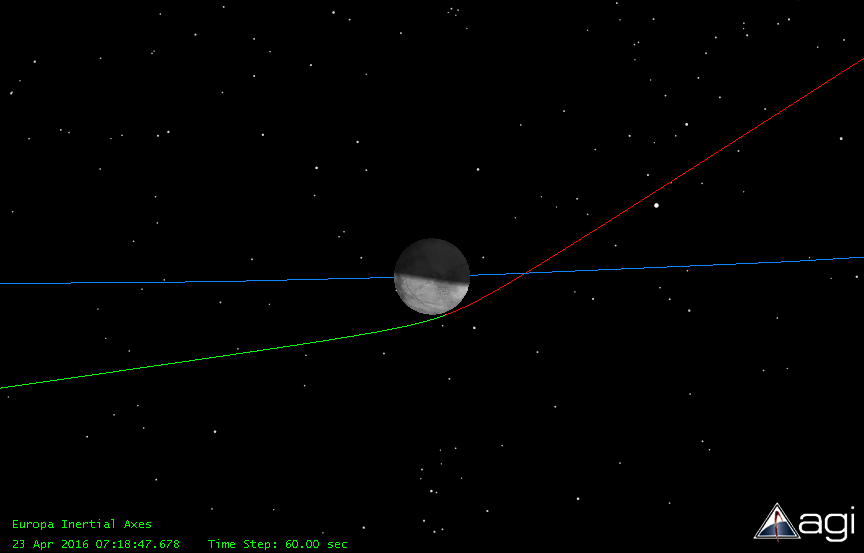
\includegraphics[width=0.9\textwidth]{figures/Orbiter/flyby2.png}
\caption{Flyby geometry targeting the trailing edge antijovian hemisphere (Ifikratis Kamenidis, STK software).}
\label{flyby2}
\end{figure}

\noindent
As the orbiter flybys Europa, the orientation of the cameras and so of the spacecraft is paramount for achieving the precise targeting. We are interested in maximizing coverage by the least amount of flybys to prolong mission life (less TID possible) as the mission goal is to land on the surface and reach the subsurface ocean by a penetrator. 
Two different imaging geometry configurations are considered. 

One solution is to implement a steady top down imaging of both narrow angle (high resolution) and wide angle (low resolution) cameras. The achieved coverage for a trailing edge inbound flyby can be seen in \ref{steadycov}. The pointing accuracy for such a configuration requires that the spacecraft will rotate in its yaw axis, based on the angular velocity of the spacecraft in respect to the Europa reference system. 

Another option is to initiate a double rotation of the spacecraft (and so the cameras). This maneuver does not pose any danger to the mission as; 1) the orbiter is powered by RTG so pointing to the sun is not necessary 2) high-gain antenna link to the Earth can be skipped for the duration of the flyby which is less than 30 minutes 3) there is no need to communicate with the lander, as the reconnaissance phase happens before lander separation. The maneuver requires the spacecraft to initiate two rotations in roll and yaw and a small pitch maneuver; First a small yaw rotation (non linear) which tracks Europa's center of gravity takes place (less than 0.1rpm - depending on flyby target radius (see figure \ref{flybyangle})) and second a roll revolution of 1 rpm. Third, placing the camera's pointing axis in an offset angle will result in a rotational effect imaging pattern. The ground area coverage for this configuration can be seen in figure \ref{rot_cover}. The angular momentum requirements can be seen in figure \ref{flybyangle} while the relative speed for a flyby aiming radius of 100Km flyby can bee seen in figure \ref{flybyspeed}.

\begin{figure}[htb!]
\centering
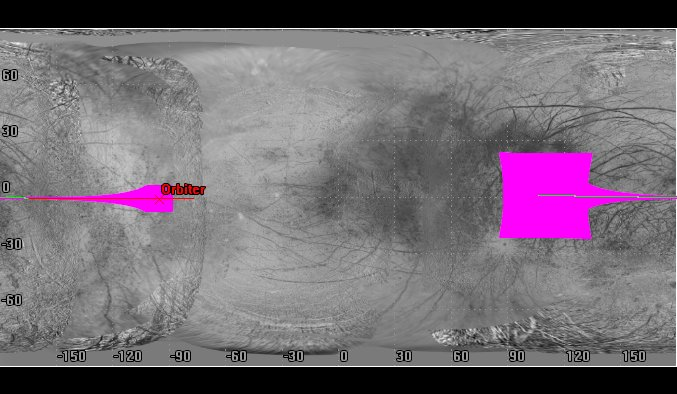
\includegraphics[width=0.9\textwidth]{figures/Orbiter/steady_cover.png}
\caption{Ground area coverage for one flyby using a steady top-down pointing. FOV:5 degrees. Inclination is zero degrees relative to Europa (Ifikratis Kamenidis, STK).}
\label{steadycov}
\end{figure}
\begin{figure}[htb!]
\centering
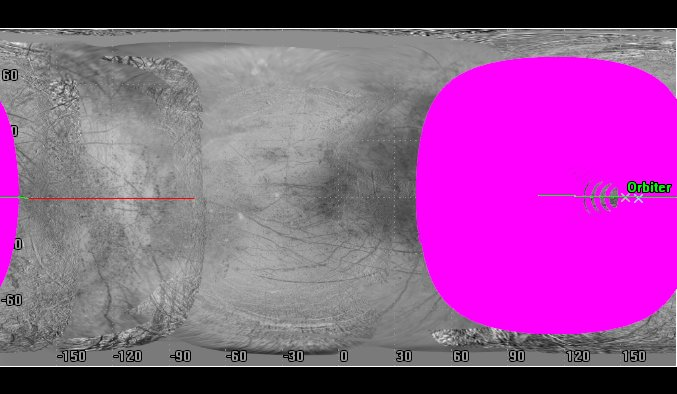
\includegraphics[width=0.9\textwidth]{figures/Orbiter/rot_cover.png}
\caption{Ground area coverage for one flyby using rotating pointing. FOV:5 degrees, rotation rate is 1rpm. Inclination is zero degrees relative to Europa(Ifikratis Kamenidis, STK).}
\label{rot_cover}
\end{figure}

\noindent
3D flyby animations of the two imaging geometries can be seen at:
\begin{description}[align=left]
\item [Steady top-down pointing:]\hfill \\
\url{https://www.youtube.com/watch?v=LjMV9DhwkUo}.
\item [Rotating pointing:]\hfill \\
\url{https://www.youtube.com/watch?v=hLvxofgHwf8}.
\end{description}


\begin{figure}[htb!]
\centering
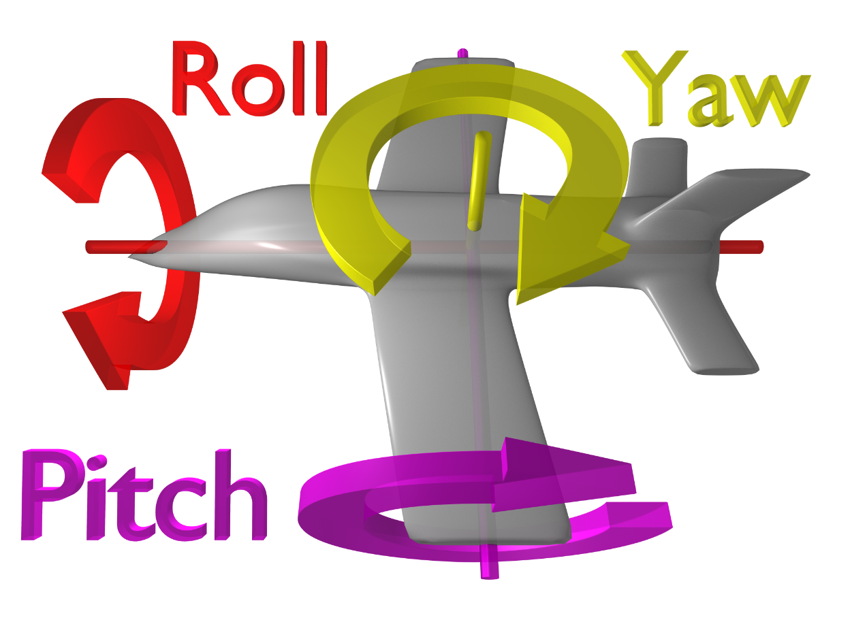
\includegraphics[scale=0.5]{figures/Orbiter/axis_o.png}
\caption[Spacecraft pitch, yaw and roll axis]{Spacecraft pitch, yaw and roll axis \footnote{wikipedia, Author:ZeroOne}.}
\label{axis_o}
\end{figure}

\begin{figure}[htb!]
\centering
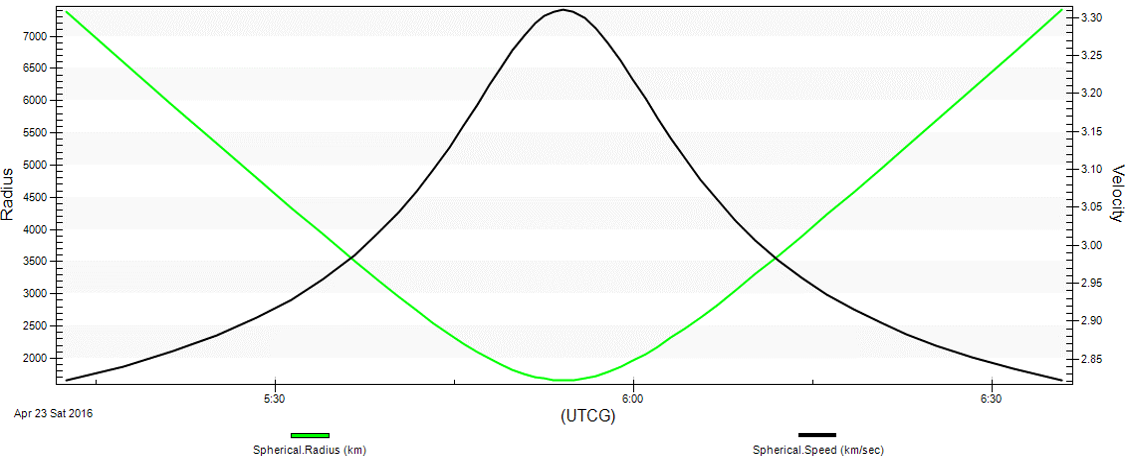
\includegraphics[width=\textwidth]{figures/Orbiter/flybyspeed.png}
\caption{Speed and Radius plot for a 100Km altitude flyby (Ifikratis Kamenidis, STK software).}
\label{flybyspeed}
\end{figure}

\begin{figure}[htb!]
\centering
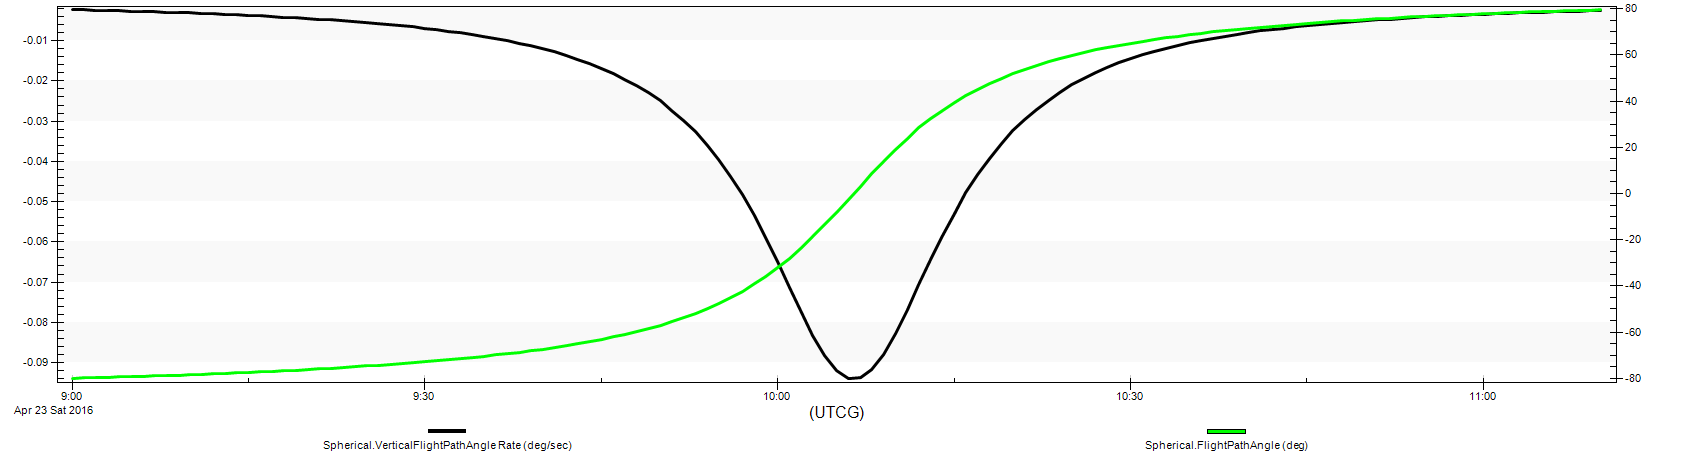
\includegraphics[width=\textwidth]{figures/Orbiter/anglerate2.png}
\caption{Angle change and angle rate for a 100Km altitude flyby (Ifikratis Kamenidis, STK software).}
\label{flybyangle}
\end{figure}